\documentclass[12pt]{article}
\title{\vspace{-2cm}Quals Study Guide}
\author{Mackenzie Lau}
\date{}
\usepackage[margin = 0.75in]{geometry}
\usepackage{graphicx, subcaption, wrapfig}
\usepackage{amsmath, amssymb, gensymb, tabularx, multirow, esint, indentfirst}
\usepackage{mathtools, bm}
\usepackage[super]{nth}
\newcommand{\Hrule}{\rule{\textwidth}{0.2mm}\\}
\newcommand{\Item}[1]{\item \textbf{#1}:}
\newcommand{\Header}[1]{\noindent\rule{\textwidth}{0.4pt}\\\large{\textit{#1}}\normalsize{}}
\newcommand{\CenteredBoxed}[1]{\begin{center}\boxed{#1}\end{center}}
\newcommand{\sumlim}[2]{\sum\limits_{#1}^{#2}}
\newcommand{\intlim}[2]{\int\limits_{#1}^{#2}}
\usepackage [english]{babel}
\usepackage [autostyle, english = american]{csquotes}
\MakeOuterQuote{"}
%% Aero commands
\newcommand{\rhoinfty}{\rho_\infty}
\newcommand{\Vinfty}{V_\infty}
\newcommand{\qinfty}{q_\infty}
\newcommand{\TSL}{T_{SL}}
\newcommand{\WTO}{W_{TO}}
%% Optimization commands
\newcommand{\boldx}{\mathbf{x}}
\newcommand{\xstar}{\boldx^*}
\newcommand{\Partial}[2]{\frac{\partial #1}{\partial #2}}
\newcommand{\PPartial}[2]{\frac{\partial^2 #1}{\partial #2^2}}
\newcommand{\PPPartial}[3]{\frac{\partial^2 #1}{\partial #2 \partial #3}}
\DeclareMathOperator{\Hessian}{Hess}
%% Thermodynamics commands
\newcommand{\PartialConst}[3]{\left(\Partial{#1}{#2}\right)_{#3}}
%% Combustion commands

\begin{document}
\maketitle
\thispagestyle{empty}
\vspace{-1cm}
\Hrule
\vspace{-1cm}
\pagestyle{empty}
\tableofcontents
\newpage
\pagestyle{plain}
\setcounter{page}{1}
\section{Fixed Wing Design}
\subsection{Basics and Background}
\begin{itemize}
\Item{Requirements Definition} A statement which identifies a system, product, or process characteristic of constraint which is unambiguous, can be verified, and is deemed necessary for stakeholder acceptability. Well-formed requirements include system functionality (capability), attributes (measurable conditions), and are bounded by constraints.
\Item{Requirement Analysis} Transform identified top-level needs and objectives into system function and performance requirements which specifically define what the system must do, how well it must perform, and what must be accomplished to ensure operational capabilities with interfacing systems are met.
\Item{What Are Requirements?} Precise statements of what must be done as well as how well and under what conditions it must be done. Delineated by the "Three C's": Capabilities, Characteristics, and Constraints.
\Item{Constraint Analysis} Ensure system can satisfy all constraints set by requirements (sizing procedure).
\Item{Mission Analysis} Analyzing system performance over a given mission (sizing procedure).
\Item{Energy-/Power-Based Analysis} Constraint diagram (carpet plot).
\Item{Layers of the Atmosphere}
	\begin{itemize}
	\Item{Troposphere} Up to 8 to 14.5 km (5 to 9 miles). Most dense, contains all weather.
	\Item{Stratosphere} Up to 50 km (31 miles). Ozone layer absorbs and scatters UV radiation.
	\Item{Mesosphere} Up to 85 km (53 miles). Meteors burn up here.
	\Item{Thermosphere} Up to 600 km (372 miles). Satellites orbit here.
	\Item{Ionosphere} Overlaps mesosphere and thermosphere, 48 to 965 km (30 to 600 miles). Makes radio communication possible.
	\Item{Exosphere} Up to 10,000 km (6,200 miles). Upper limit of atmosphere.
	\end{itemize}
\Item{Standard Atmosphere} 66.2\degree F (19\degree C), 1.075 atm (108.9 kPa), 0.0025195 $slug/ft^3$ (1.2985 $kg/m^3$)
\Item{Temperature Lapse} Troposphere: approx -18.8\degree F per mile (-6.5\degree C per km). Stratosphere: approx. +2.89\degree F per mile (+1.0\degree C per km)
\end{itemize}

\subsection{Aerodynamics}
\subsubsection{Fundamentals of Fluid Dynamics}
\begin{itemize}
\Item{Inviscid Flow} Zero viscosity ($Re = \infty$)
\Item{Incompressible Flow} Constant density
\Item{Bernoulli's Equation} $p + \frac{1}{2}\rho V^2 = const.$\\
	\begin{itemize}
	\item Start from general momentum equation $\rho\frac{Du}{Dt} = \sum F''' = -\frac{\partial p}{\partial x}+ \rho f_x + f_v$, ignoring body and viscous forces. Assume, without loss of generality, we are in the $x$ direction
	\item Write out substantial derivative $\rho\frac{Du}{Dt} = \rho\left(\frac{\partial u}{\partial t} + u\frac{\partial u}{\partial x} + v\frac{\partial u}{\partial y} + w\frac{\partial u}{\partial z}\right)$. Assuming steady flow $\frac{\partial u}{\partial t} = 0$
	\item Substitute, multiply both sides by $dx$, and simplify by applying to a stream (such that $udz=wdx$ and $udy=vdx$) to get $u\left(\frac{\partial u}{\partial x}dx+\frac{\partial u}{\partial y}dy+\frac{\partial u}{\partial z}dz\right)=\frac{-1}{\rho}\frac{\partial p}{\partial x}dx$
	\item Recognize the term in parentheses on the right hand side is the differential of the $x$-component of the velocity $du = \frac{\partial u}{\partial x}dx+\frac{\partial u}{\partial y}dy+\frac{\partial u}{\partial z}dz$
	\item Substitute to get $udu = \frac{-1}{\rho}\frac{\partial p}{\partial x}dx$
	\item Repeat for $y$ and $z$ directions
	\item Recognize the sum of squares of the velocity components is the square of the velocity itself ($u^2+v^2+w^2=V^2$)
	\item Recognize the sum of the partial derivatives of pressure in each direction multiplied by the component differential is the differential of the pressure ($\sum\frac{\partial p}{\partial x_i}dx_i = dp$)
	\item Arrive at Euler's equation: $\frac{1}{2}d(V^2) = \frac{-dp}{\rho}\implies$ \boxed{dp = -\rho VdV}. Euler's equation applies to \textit{any} steadily flowing fluid
	\item Apply Euler's equation to a streamline assuming constant density (incompressible flow) and integrate between two states to get Bernoulli's equation 
	$$\intlim{p_1}{p_2}dp = -\rho\intlim{V_1}{V_2}VdV$$
	$$p_2-p_1 = \rho\left(\frac{1}{2}V_1^2 - \frac{1}{2}V_2^2\right)$$
	$$p_1 + \frac{1}{2}\rho V_1^2 = p_2 + \frac{1}{2}\rho V_2^2$$
	\CenteredBoxed{p+\frac{1}{2}\rho V^2 = const.}
	\item Bernoulli's equation applies to any individual stream line, indepent of whether or not the flow is rotational. In the special case of irrotational flow ($\nabla\times V = 0$) the constant is the same for each streamline, thus Bernoulli's equation holds for the entire flow field, not just a streamline.
	\end{itemize}
\Item{Irrotational Flow} A flow is irrotational if individual fluid elements do not rotate about their centers of gravity; the fluid elements poses no angular velocity and their motion through space is pure translation ($\nabla\times V = 0$ throughout the fluid). Inviscid flow may be either rotational or irrotational. Viscous flow must be rotational.
\Item{Circulation} $\Gamma\equiv-\oint V\cdot ds=\varointclockwise V\cdot ds$ (circulation is taken to be positive clockwise for convenience). Circulation does \emph{not} imply the fluid elements are doing circuits; rather, circulation in the context of aerodynamics means the closed-loop integral is finite. Applying Stoke's theorem yields $-\frac{d\Gamma}{dS} = (\nabla\times V)\cdot\mathbf{n}$ where $\mathbf{n}$ is the normal to the open surface which bounds the curve around which $V\cdot ds$ is integrated.
\Item{Stream Function} Two-dimensional steady flow yields the equation $\frac{dy}{dx} = \frac{v}{u}$ for a streamline. With $v$ and $u$ known functions of $x$ and $y$, we can write the stream function $\bar{\psi}(x,y) = c$
	\begin{itemize}
	\item Since the velocity vector at any point is tangent to the stream line at that point (i.e. there is no normal velocity) the mass flux between any two stream lines must remain constant throughout the flow field (for incompressible flow). This means local velocity is inversely proportional to stream line spacing at any point in the flow
	\item We can also deduce the following
	$$ \Delta\bar{\psi}\equiv\rho V\Delta n(unit\ depth\ into\ page)$$
	$$\lim_{\Delta n\to0}\frac{\Delta\bar{\psi}}{\Delta n}\equiv\frac{\partial\bar{\psi}}{\partial n} = \rho V$$
	$$\mathrm{Conservation of mass}\implies\rho V\Delta n = \rho u\Delta y - \rho v\Delta x$$
	$$d\bar{\psi} = \rho udy - \rho vdy$$
	$$\mathrm{By the chain rule}\ \bar{\psi} = \bar{\psi}(x,y) \implies d\bar{\psi} = \frac{\partial\bar{\psi}}{\partial x}dx + \frac{\partial\bar{\psi}}{\partial y}dy$$
	\CenteredBoxed{\rho u = \frac{\partial\bar{\psi}}{\partial x}\to u=\frac{\partial\psi}{\partial x},\quad \rho v = -\frac{\partial\bar{\psi}}{\partial y}\to v=-\frac{\partial\psi}{\partial y}}
	\item Polar coordinates: $u_r=\frac{1}{r}\frac{\partial\psi}{\partial \theta}$, $u_\theta=-\frac{\partial\psi}{\partial r}$
	\end{itemize}
\Item{Velocity Potential} If $\xi = \nabla\times V = 0$ then $\exists\phi=\phi(x,y,z):\mathbb{R}^3\to\mathbb{R}\ s.t.\ \nabla\times(\nabla\phi)=0$ and $V=\nabla\phi$
	\begin{itemize}
	\item As a direct consequence, $u=\frac{\partial\phi}{\partial x}$, $v=\frac{\partial\phi}{\partial y}$, $w=\frac{\partial\phi}{\partial z}$ (from definition of Cartesian gradient)
	\item Cylindrical coordinates: $u_r=\frac{\partial\phi}{\partial r}$, $u_\theta=\frac{1}{r}\frac{\partial\phi}{\partial \theta}$, $u_z=\frac{\partial\phi}{\partial z}$
	\item Spherical coordinates: $u_r=\frac{\partial\phi}{\partial r}$, $u_\theta=\frac{1}{r}\frac{\partial\phi}{\partial \theta}$, $u_\Phi=\frac{1}{r\sin\theta}\frac{\partial\phi}{\partial \Phi}$, 
	\end{itemize}
\Item{Vortex Sheet Strength} $\Gamma = \intlim{a}{b}\gamma ds$
	\begin{itemize}
	\item Local vortex strength is equal to the local velocity discontinuity ($\gamma=u_1-u_2$)
	\item Kutta-Joukowski Theorem: $L' = \rhoinfty \Vinfty\Gamma$
	\item Kutta Condition $\implies (\gamma(TE) = 0)\ ||\ (\gamma(TE) = \mathrm{finite}\implies V_1=V_2\neq0)$
	\item Kelvin's Circulation Theorem: $\frac{D\Gamma}{Dt} = 0$, i.e. in inviscid, incompressible flow, the circulation around a closed curve consisting of the same fluid elements does not change with time. This leads to the starting and shed vortex theories.
	\end{itemize}
\end{itemize}
\subsubsection{Two-Dimensional Aerodynamics}
\Header{Fundamentals}
\begin{itemize}
\Item{Purpose of an Airfoil} Generate lift
\Item{Draw an Airfoil}
\Item{NACA 4 Series} \nth{1} = max camber as percent of chord; \nth{2} = location of max camber as percent of chord; \nth{3}-\nth{4} = max thickness as percent of chord
\Item{NACA 5 Series} \nth{1} = two-thirds design $c_l$, in tenths; \nth{2} = location of max camber, in fifths; \nth{3} = reflex camber; \nth{4}-\nth{5} = thickness as percent of chord
\Item{NACA 6 Series} \nth{1} = 6 (series ID); \nth{2} = location of minimum pressure, in tenths of percent of chord; \nth{3} = design lift coefficient, in tenths; \nth{4}-\nth{5} = max thickness as percent of chord
\Item{Lift Coefficient} $c_l \equiv \frac{L'}{qc},\ q = \frac{1}{2}\rho \Vinfty^2$
\Item{Drag Coefficient} $c_d \equiv \frac{D'}{qc}$
\Item{Moment Coefficient} $c_m \equiv \frac{M'}{qc^2}$
\Item{Pressure Coefficient} $C_p \equiv \frac{p-p_\infty}{\qinfty} = 1-\left(\frac{V}{\Vinfty}\right)^2$
\Item{Velocity Induced by a Vortex} $V_\theta = -\frac{\Gamma}{2\pi r}$
	\begin{itemize}
	\item $dV_\theta = -\frac{\gamma(\xi)d\xi}{2\pi r}$
	\end{itemize}
\Item{D'Alembert's Paradox} A two-dimensional body in potential flow will experience no drag. This is a direct result of the potential flow assumption as drag (mostly) a viscous phenomenon
\end{itemize}

\Header{Thin Airfoil Theory}
\begin{itemize}
\Item{Induced Velocity} $w'=w'(s)$ is the velocity normal to the camber line induced by the vortex sheet
\Item{Camber Line vs Chord Line} May approximate the two as equal for thin airfoils of moderate camber when viewed from a distance. That is, camber $<<$ chord. This allows us to write $\gamma=\gamma(x)$. We do, however, wish to maintain the camber line as a streamline (though the chord line need not be)
\Item{Camber Line as Streamline} Require the local induced velocity to be equal and opposite in direction to the normal component of the free stream velocity
$$V_{\infty,n} +w'(s) = 0, \quad V_{\infty,n} = \Vinfty\sin\left[\alpha+\arctan\left(-\frac{dz}{dx}\right)\right]$$
For a thin airfoil at a small angle of attack, the camber line $\approx$ chord line assumption can be applied again along with the small angle approximation for sines and cosines to arrive at
$$V_{\infty,n} \approx \Vinfty\left(\alpha-\frac{dz}{dx}\right)$$
Furthermore, the camber line $\approx$ chord line assumption lets us rewrite the induced velocity as
$$w'(s)\approx w'(x)$$
By applying the integral form of the velocity induced at a point by a vortex sheet we can write
$$w'(x) = -\intlim{0}{c}\frac{\gamma(\xi)d\xi}{2\pi(x-\xi)}$$
Substituting the assumptions we've made into the first equation we get\\
\CenteredBoxed{\Vinfty\left(\alpha-\frac{dz}{dx}\right)=\intlim{0}{c}\frac{\gamma(\xi)d\xi}{2\pi(x-\xi)}}
\Item{Thin, Symmetric Airfoil} $\frac{dz}{dx}=0$, parameterize $\xi$ in terms of $\theta$ to simplify integration
$$ \xi = \frac{c}{2}\left(1-\cos\theta\right),\quad x = \frac{c}{2}\left(1-\cos\theta_0\right),\quad d\xi = \frac{c}{2}\sin\theta d\theta$$
$$\frac{1}{2\pi}\intlim{0}{\pi}\frac{\gamma(\theta)\sin\theta d\theta}{\cos\theta-\cos\theta_0}=\Vinfty\alpha$$
\CenteredBoxed{\gamma(\theta)=2\alpha \Vinfty\frac{1+\cos\theta}{\sin\theta}}
Application of L'Hospital's rule shows $\gamma(\pi) = 2\alpha \Vinfty\frac{-\sin\pi}{\cos\pi}=0$
\Item{Lift in terms of Circulation} Find $\Gamma$ by integrating $\gamma(\xi)$
$$\Gamma = \intlim{0}{c}\gamma(\xi)d\xi = \frac{c}{2}\intlim{0}{\pi}\gamma(\theta)\sin\theta d\theta$$
\CenteredBoxed{\Gamma = \alpha c\Vinfty\intlim{0}{\pi}(1+\cos\theta)d\theta = \pi\alpha c\Vinfty}
Then, by the definition of the lift coefficient,
\CenteredBoxed{c_l\equiv\frac{L'}{qc}=\frac{\rhoinfty \Vinfty(\pi\alpha c\Vinfty)}{\frac{1}{2}\rhoinfty \Vinfty^2c}=2\pi\alpha}
\CenteredBoxed{\frac{dc_l}{d\alpha} = 2\pi\ \textrm{per radian}}
\Item{Moment Coefficient} Lift creates a moment about the leading edge. Consider an elemental vortex of strength $\gamma(\xi)d\xi$ located at a distance $\xi$ from the leading edge. Then the circulation associated with the elemental vortex is $d\Gamma = \gamma(\xi)d\xi$, resulting in an increment in lift $dL' = \rhoinfty \Vinfty d\Gamma$. The resulting lift generates a moment about the leading edge $dM_{LE}=-\xi dL'$. Then the total moment about the leading edge is given by
\CenteredBoxed{M'_{LE} = -\intlim{0}{c}\xi dL'=-\rhoinfty \Vinfty\intlim{0}{c}\xi\gamma(\xi)d\xi = -\qinfty c^2\frac{\pi\alpha}{2}}
Then the moment coefficient is given by
\CenteredBoxed{c_{m,LE}=\frac{M'_{LE}}{\qinfty c^2}=-\frac{\pi\alpha}{2}=-\frac{c_l}{4}}
\Item{Moment Coefficient about Quarter-Chord for Symmetric Airfoil} The moment about the quarter-chord is given by (the right hand side of the implication is found by dividing both sides by $\qinfty Sc$ with $S=c(1)$, hence the $c$ dropping from the lift coefficient):
$$M'_{c/4}=M'_{LE}+\frac{c}{4}L' \implies c_{m,c/4}=c_{m,LE}+\frac{1}{4}c_l$$
Thus the moment cofficient about the quarter-chord for a symmetric airfoil is
\CenteredBoxed{c_{m,c/4}=-\frac{c_l}{4}+\frac{c_l}{4}=0}
Thus the center of pressure for a symmetric airfoil lies at the quarter-chord point. Furthermore, the aerodynamic center is very near the quarter-chord point for symmetric airfoils at moderate angles of attack.
\Item{Cambered Airfoils} The general results of $\frac{dc_l}{d\alpha}=2\pi$ holds, but there is a difference in the integral term in the expression for $c_l$
$$c_l=2\pi\left[\alpha+\frac{1}{\pi}\intlim{0}{\pi}\frac{dz}{dx}(\cos\theta_0-1)d\theta_0\right]$$
Physically, the integral term represents the \emph{zero-lift angle of attack} for a cambered airfoil.
$$\alpha_{L=0}=-\frac{1}{\pi}\intlim{0}{\pi}\frac{dz}{dx}(\cos\theta_0-1)d\theta_0$$
This equation implies airfoils with greater camber have more-negative zero-lift angles of attack. Also, the degenerate case where $\frac{dz}{dx}=0$ reduces to the result for symmetric airfoils ($\alpha_{L=0}=0$).
\Item{More on Cambered Airfoils} The above analyses were carried out by solving for $\gamma(\theta)$ as a Fourier sine series and taking advantage of integral rules with regard to produces of trigonometric functions (review numerical solutions to partial differential equations if you're really curious). The preceding analyses find the circulation around a cambered airfoil as
\CenteredBoxed{\Gamma=c\Vinfty\left(\pi A_0+\frac{\pi}{2}A_1\right)}
$$A_0=\alpha-\frac{1}{\pi}\intlim{0}{\pi}\frac{dz}{dx}d\theta_0$$
$$A_n=\frac{2}{\pi}\intlim{0}{\pi}\frac{dz}{dx}\cos(n\theta_0)d\theta_0$$
Another important result which falls out from this analysis is that for the leading edge moment coefficient
\CenteredBoxed{c_{m,le}=-\left[\frac{c_l}{4}+\frac{\pi}{4}(A_1-A_2)\right]}
which leads directly to the quarter-chord moment coefficient and the center of pressure location
\CenteredBoxed{c_{m,c/4}=\frac{\pi}{4}(A_2-A_1)\to x_{cp}=\frac{c}{4}\left[1+\frac{\pi}{c_l}(A_1-A_2)\right]}
This suggests the center of pressure moves to infinity as a cambered airfoil approaches the zero-lift angle of attack
\end{itemize}

\Header{Practical Airfoil Theory}
\begin{itemize}
\Item{Center of Pressure} The center of pressure $x_{cp}$ is the location at which the airfoil generates lift but no moment ($c_{m,cp}=0$). It is found via
\CenteredBoxed{x_{cp}=\frac{c}{4}-\frac{M'_{c/4}}{L'}=c\left(\frac{1}{4}-\frac{c_{m,c/4}}{c_l}\right)}
\Item{Aerodynamic Center} The point about which the aerodynamic moment is independent of angle of attack ($\frac{dc_m}{d\alpha}=0$). The aerodynamic center of an airfoil can be found via
\CenteredBoxed{\bar{x}_{ac}=0.25-\frac{m_0}{a_0}}
where $m_0=\frac{dc_{m,c/4}}{d\alpha}$ and $a_0=\frac{dc_l}{d\alpha}$. Note the subtle difference between this expression and that for the center of pressure
\Item{Vortex Panel Method} An extension of the vortex sheet method. Apply vortex sheet theory to segments of an arbitrary lifting body (i.e. not just thin airfoils).
\Item{Skin Friction Coefficient} 
	\begin{itemize}
	\item Laminar: $C_f=\frac{1.328}{\sqrt{Re_c}}$
	\item Turbulent: $C_f=\frac{0.074}{Re_c^{1/5}}$
	\end{itemize}
\Item{Critical Reynolds Number} Transition typically occurs in the vicinity of $5\times10^5$ for external flow. Given the flow velocity and assuming typical air properties ($\mu\approx1.8\times10^{-5}\ kg/(ms)$ and $\rhoinfty=1.23\ kg/m^2$), one can find the transition distance $x_{cr}$
\Item{Flow Separation} Drastic loss of lift and significant increase in (pressure) drag. Caused by adverse pressure gradients and the flows inability to overcome those gradients. Trailing edge stall is less severe than leading edge stall (albeit with a lower maximum lift coefficient)
\Item{High Lift Devices} Flaps and slats are the main methods for increasing lift. Without high lift devices, a wing would have to be sized for takeoff and landing (low speed events) and performance would suffer during cruise (high speed condition). More on this later
\end{itemize}

\subsubsection{Three-Dimensional Aerodynamics -- Lift}
\begin{itemize}
\Item{Finite Wing} Pressure difference between top and bottom surfaces alters the flow. Over the top surface there is a spanwise flow inwards (towards the root) while along the bottom surface there is a spanwise flow outward (towards the tip). Tip vortices form as a result of high pressure bottom surface flow leaking around the tip to the low pressure top surface
\Item{Biot-Savart Law} The velocity at a point induced by a vortex filament is given by
\CenteredBoxed{\mathbf{dV}=\frac{\Gamma}{4\pi}\frac{\mathbf{dl}\times\mathbf{r}}{|\mathbf{r}|^3}}
Applying this to an infinitely long, straight vortex filament and integrating yields
\CenteredBoxed{V_{induced}=\frac{\Gamma}{2\pi h}}
\Item{Prandtl's Lifting Line} Represent the finite wing as an infinite number of horseshoe vortices which tail off to infinity behind the airfoil (representation below)
\begin{figure}[h]
\centering
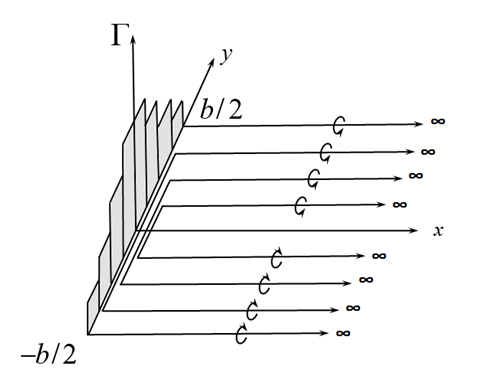
\includegraphics[scale=0.5]{Graphics/horseshoe_vortex.png}
\end{figure}
\Item{Induced Velocity} The downwash at any point $y_0$ is given by
\CenteredBoxed{w(y_0)=-\frac{1}{4\pi}\intlim{-b/2}{b/2}\frac{(d\Gamma/dy)dy}{y_0-y},\ \Gamma=\Gamma(y)}
\Item{Induced Angle of Attack} The induced angle of attack at a location $y_0$ is
$$\alpha_i(y_0)=\arctan\left(\frac{-w(y_0)}{\Vinfty}\right)$$
Substituting the equation for the induced velocity and assuming the magnitude of the induced velocity is much less than that of the free stream velocity (small angle approximation for $\tan$) yields the result
\CenteredBoxed{\alpha_i(y_0) =\frac{1}{4\pi\Vinfty}\intlim{-b/2}{b/2}\frac{(d\Gamma/dy)dy}{y_0-y}}
The induced angle of attack \emph{reduces} the effective angle attack from the geometric angle of attack. It has the effect of tilting the lift vector back (downstream), which reduces lift by $L\cos\alpha_i$ and increases drag by $L\sin\alpha_i$. See illustration below
\begin{figure}[h]
\centering
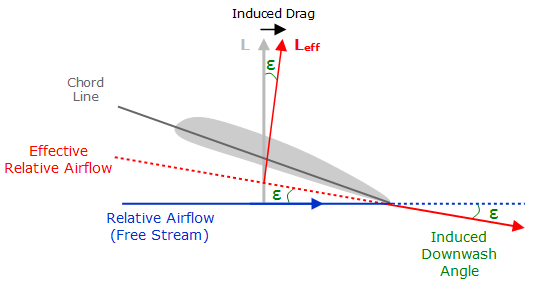
\includegraphics[scale=0.5]{Graphics/induced_diagram.png}
\end{figure}
\Item{Elliptic Lift Distribution} The elliptic lift distribution (not elliptic planform) is the special case of the minimum induced drag and constant downwash (and thus constant induced angle of attack). The distribution is expressed through the elliptic circulation distribution as
$$\Gamma(y)=\Gamma_0\sqrt{1-\left(\frac{2y}{b}\right)^2}$$
through with the lift distribution can be written as
$$L'(y)=\rhoinfty\Vinfty\Gamma_0\sqrt{1-\left(\frac{2y}{b}\right)^2}$$
Find the slope of the circulation distribution as
$$\frac{d\Gamma}{dy}=-\frac{4\Gamma_0}{b^2}\frac{y}{(1-4y^2/b^2)^{1/2}}$$
and integrate such that the induced velocity at a location $\theta_0$ -- parameterization in terms of $\theta$ simplifies integration -- is given by
$$w(\theta_0)=-\frac{\Gamma_0}{2b} = w$$
So the induced angle of attack is given by
$$\alpha_i=-\frac{w}{\Vinfty}=\frac{\Gamma_0}{2b\Vinfty}$$
After integrating the lift distribution and applying the definition of the lift coefficient we arrive at the result
$$ \frac{1}{2}\rhoinfty\Vinfty^2SC_L=L=\rhoinfty\Vinfty\Gamma_0\frac{b}{4}\pi$$
$$\Gamma_0=\frac{2\Vinfty SC_L}{b\pi}$$
\CenteredBoxed{\alpha_i=\frac{C_L}{\pi AR}}
We can then obtain the induced drag from the relation $D_i'=L'\alpha_i$, where the small angle approximation was used, as
\CenteredBoxed{C_{D,i}=\frac{C_L^2}{\pi AR}}
\Item{Oswald Efficiency Factor} The induced drag for a general lift distribution is given by
\CenteredBoxed{C_{D,i}=\frac{C_L^2}{\pi eAR},\ e\leq1}
or, more directly
\CenteredBoxed{C_{D,i}=\frac{C_L^2}{\pi AR}(1+\delta),\ \delta=\sum\limits_2^n n(A_n/A_1)^2\geq0}
The induced drag factor $\delta$ varies with wing geometry (see below)
\begin{figure}[h]
\centering
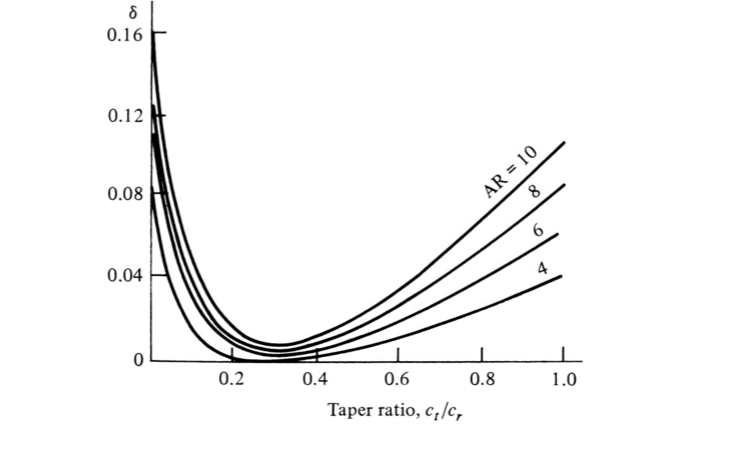
\includegraphics[scale=0.4]{Graphics/delta_vs_lambda.png}
\end{figure}
\Item{Effect of Induced AoA on Lift Curve} The induced angle of attack, being a function of the lift coefficient, has a tendency to reduce the slope of the lift curve. The manner in which it does this is given by
$$\frac{dC_L}{d(\alpha-\alpha_i)}=a_0\implies C_L=a_0(\alpha-\alpha_i)+\mathrm{const}$$
Substituting the result for the induced angle of attack, differentiating and solving for the lift curve slope again, then generalizing the planform gives
$$\frac{dC_L}{d\alpha}=a=\frac{a_0}{1+(a_0/\pi AR)(1+\tau)},\ \tau\in[0.05+0.25]$$
\Item{Vortex Lattice Method} Lifting line theory breaks down for low aspect ratio wings, swept wings, and delta wings. For low AR wings, the tip vortices start to cover a significant portion of the wing. Vortex lattice theory, a panel method, generalizes lifting line theory to be applicable to these cases. The following results are obtained from these modifications (for incompressible flow only):

Low aspect ratio ($AR<4$), straight wing
\CenteredBoxed{a=\frac{a_0}{\sqrt{1+(a_0/\pi AR)^2}+a_0/\pi AR}}

Swept wing ($\Lambda = $  angle of half-chord line with horizontal)
\CenteredBoxed{a=\frac{a_0\cos\Lambda}{\sqrt{1+(a_0\cos\Lambda/\pi AR)^2}+a_0\cos\Lambda/\pi AR}}
\Item{Vortex Lift} Flow will tend to separate along the leading edge of a delta wing (if the LE is sharp) and reattach further down the wing. The high energy vortex has low \emph{static} pressure. This suction effect generates lift at high angles of attack (angles at which conventional wings would stall). A significant portion of the lift is generated near the leading edge of the delta.
\end{itemize}

\subsubsection{Three-Dimensional Aerodynamics -- Drag}

\subsection{Performance}
\subsubsection{Equations of Motion} 
\begin{center}\textbf{\emph{DRAW THE DIAGRAMS}}\end{center}
\CenteredBoxed{m\frac{d\Vinfty}{dt}=T\cos\varepsilon-(D+W\sin\theta)}
\CenteredBoxed{m\frac{\Vinfty^2}{R_1}=(L+T\sin\varepsilon)\cos\phi-W\cos\theta}
\CenteredBoxed{m\frac{(\Vinfty\cos\theta)^2}{R_2}=(L+T\sin\varepsilon)\sin\phi}
\subsubsection{Mattingly's Master Equation}
\CenteredBoxed{\frac{\TSL}{\WTO}=\frac{\beta}{\alpha}\left[\frac{\qinfty S}{\beta\WTO}\left(C_{D,0}+\frac{nk_1\beta}{\qinfty}\left(\frac{\WTO}{S}\right)+\frac{n^2k_2\beta^2}{\qinfty^2}\left(\frac{\WTO}{S}\right)^2+\frac{R}{\qinfty S}\right) + \frac{1}{\Vinfty}\frac{d}{dt}\left(h+\frac{\Vinfty^2}{2g}\right)\right]}

Derivation:
$$P_s = \dot{z}_e=\frac{d}{dt}\left(mgh+\frac{1}{2}m\Vinfty^2\right)$$
$$\frac{P_s}{W}=\frac{d}{dt}\left(h+\frac{\Vinfty^2}{2g}\right)$$
$$\frac{(T-D-R)\Vinfty}{W}=\frac{d}{dt}\left(h+\frac{\Vinfty^2}{2g}\right)$$
$$\frac{T}{W}=\frac{1}{W}\left(D+R\right)+\frac{1}{\Vinfty}\frac{d}{dt}\left(h+\frac{\Vinfty^2}{2g}\right)$$
$$D=\qinfty SC_D=\qinfty S\left(C_{D,0}+k_1C_L+k_2C_l^2\right)$$
$$C_L=\frac{L}{\qinfty S}=\frac{nW}{\qinfty S}$$
$$\frac{T}{W}=\frac{\qinfty S}{W}\left(C_{D,0}+k_1\frac{nW}{\qinfty S}+k_2\left(\frac{nW}{\qinfty S}\right)^2 +\frac{R}{\qinfty S}\right)+\frac{1}{\Vinfty}\frac{d}{dt}\left(h+\frac{\Vinfty^2}{2g}\right)$$
$$W=\beta\WTO,\quad T=\alpha\TSL$$
$$Q.E.D.$$
\subsubsection{Master Equation Responses}
\begin{itemize}
\Item{Terms} Master equation consists of constant, inverse, and linear terms
$$\frac{\TSL}{\WTO}\approx a_0 + a_1\left(\frac{\WTO}{S}\right)^{-1}+a_2\left(\frac{\WTO}{S}\right)$$
\end{itemize}
\subsubsection{Turn Radii}
Turn radius can be calculated from the load factor or vice versa via the equations of motion. Assuming thrust is aligned with the free stream ($\varepsilon=0$) for a steady level turn
\CenteredBoxed{m\frac{\Vinfty^2}{R_2}=nmg\sin\phi\implies R_2=\frac{\Vinfty^2}{ng\sin\phi}}
$$n=\frac{1}{\cos\phi}\implies\frac{1}{n^2}+\sin^2\phi = 1\implies R_2 = \frac{\Vinfty^2}{g\sqrt{n^2-1}}$$
\CenteredBoxed{\omega=\frac{\Vinfty}{R_2} = \frac{g\sqrt{n^2-1}}{\Vinfty}}
$$T=D=\qinfty S\left[C_{D,0}+K\left(\frac{nW}{\qinfty S}\right)^2\right]$$
\CenteredBoxed{n=\left[\frac{\qinfty}{K(W/S)}\left(\frac{T}{W}-\frac{\qinfty C_{D,0}}{W/S}\right)\right]^{1/2}=\left[\frac{\qinfty}{K(W/S)}\frac{P_s}{W}\right]^{1/2}}
\subsubsection{Range}

\Header{Thrust-Rated Aircraft}
\CenteredBoxed{R=\left(\frac{L}{D}\right)\left(\frac{\Vinfty}{TSFC}\right)\ln\frac{W_i}{W_f}}
Maximum Range: Assume $\Vinfty$ varies such that $L=W$ with constant $C_L$
$$\Vinfty=\sqrt{\frac{W}{\qinfty SC_L}},\ L=\qinfty SC_L,\ D=\qinfty SC_D$$
\CenteredBoxed{R\propto\frac{C_L^{1/2}}{C_D}}
$$\left(\frac{C_L^{1/2}}{C_D}\right)_{max}\implies\frac{d}{dC_L}\frac{C_L^{1/2}}{C_D}=0$$
$$\frac{d}{dC_L}\frac{C_L^{1/2}}{C_D}=0\implies\frac{1}{2}C_L^{-1/2}(C_{D,0}+KC_L^2)-2C_L^{1/2}(KC_L)=0$$
$$C_L=\sqrt{\frac{C_{D,0}}{3K}}\implies C_D=\frac{4}{3}C_{D,0}$$
\CenteredBoxed{\left(\frac{C_L}{C_D}\right)_{\left(\frac{C_L^{1/2}}{C_D}\right)_{max}}=\frac{3}{4}\sqrt{\frac{1}{3KC_{D,0}}}}

\Header{Power-Rated Aircraft}
\CenteredBoxed{R=\left(\frac{L}{D}\right)\left(\frac{\eta}{c}\right)\ln\frac{W_i}{W_f}}
Maximum Range:
\CenteredBoxed{R\propto\frac{C_L}{C_D}}
$$\left(\frac{C_L}{C_D}\right)_{max}\implies\frac{d}{dC_L}\frac{C_L}{C_D}=0$$
$$\frac{d}{dC_L}\frac{C_L}{C_D}=0\implies(C_{D,0}+KC_L^2)-2C_L(KC_L)=0$$
$$C_L=\sqrt{\frac{C_{D,0}}{K}}\implies C_D=2C_{D,0}$$
\CenteredBoxed{\left(\frac{C_L}{C_D}\right)_{max}=\sqrt{\frac{1}{4KC_{D,0}}}}
\subsubsection{Endurance}
\Header{Thrust-Rated Aircraft}
\CenteredBoxed{E=\left(\frac{L}{D}\right)\left(\frac{1}{TSFC}\right)\ln\frac{W_i}{W_f}}
Maximum Endurance:
\CenteredBoxed{E\propto\frac{C_L}{C_D}}
\CenteredBoxed{\left(\frac{C_L}{C_D}\right)_{max}=\sqrt{\frac{1}{4KC_{D,0}}}}

\Header{Power-Rated Aircraft}
\CenteredBoxed{E=\left(\frac{L}{D}\right)\left(\frac{\eta}{c\Vinfty}\right)\ln\frac{W_i}{W_f}}
Maximum Endurance: Assume $\Vinfty$ varies such that $L=W$ with constant $C_L$
$$\Vinfty=\sqrt{\frac{W}{\qinfty SC_L}},\ L=\qinfty SC_L,\ D=\qinfty SC_D$$
\CenteredBoxed{E\propto\frac{C_L^{3/2}}{C_D}}
$$\left(\frac{C_L^{3/2}}{C_D}\right)_{max}\implies\frac{d}{dC_L}\frac{C_L^{3/2}}{C_D}=0$$
$$\frac{d}{dC_L}\frac{C_L^{3/2}}{C_D}=0\implies\frac{3}{2}C_L^{1/2}(C_{D,0}+KC_L^2)-2C_L^{3/2}(KC_L)=0$$
$$C_L=\sqrt{\frac{3C_{D,0}}{K}}\implies C_D=4C_{D,0}$$
\CenteredBoxed{\left(\frac{C_L}{C_D}\right)_{\left(\frac{C_L^{3/2}}{C_D}\right)_{max}}=\frac{1}{4}\sqrt{\frac{3}{KC_{D,0}}}}

\Header{Wind Effects}\\

For the \emph{same airspeed}, headwind reduces ground speed while tailwind increases ground speed. Mark off the airspeed corresponding to zero ground speed on the $D-V$ plot and draw tangents.\\

\subsubsection{Rate of Climb}
Unaccelerated, climbing flight
$$T-D-W\sin\theta=m\frac{d\Vinfty}{dt}=0$$
$$L-W\cos\theta=m\Vinfty\frac{d\theta}{dt}=0$$
\CenteredBoxed{\frac{dh}{dt}=\Vinfty\sin\theta=\frac{T-D}{W}}

The climb angle $\theta$ is found as
$$\theta=\arcsin\left(\frac{T-D}{W}\right)$$
For turbine-driven aircraft, thrust is (mostly) independent of airspeed. Thus the maximum climb angle occurs at the minimum drag condition. The maximum rate of climb, however, occurs at the minimum required power condition (minimum $D\Vinfty$).

\subsubsection{Power Required}
\CenteredBoxed{P_{req}=D\Vinfty=\frac{1}{2}\rhoinfty\Vinfty^3SC_{D,0}+\frac{2KW^2}{\rhoinfty\Vinfty S}}
Graphically, minimum $\frac{P_{req}}{\Vinfty}$ corresponds with minimum $D$ condition.
\subsubsection{Gliding Flight}
Assume steady, gliding flight (unpowered). Then, for a glide angle $\theta$
$$L=W\cos\theta$$
$$D=W\sin\theta$$
\CenteredBoxed{\left(\frac{L}{D}\right)^{-1}=\tan\theta}
Glide range can be calculated assuming a constant glide angle
$$R=\frac{\Delta h}{\tan\theta}=\frac{L}{D}\Delta h$$
Thus maximum range corresponds to the maximum $L/D$ and, consequently, the minimum glide angle. The minimum sink rate, however, does not correspond to the minimum range. The minimum sink rate is found by
$$\dot{h}=-\Vinfty\sin\theta,\ \sin\theta=\frac{D}{W}=\frac{D}{L}$$
where the last equality was made with the small angle approximation for the glide angle. Then the minimum sink rate corresponds to the minimum power condition
\CenteredBoxed{\dot{h}_{min}\propto\frac{C_D}{C_L^{3/2}}}
this should make sense as the sink rate can be equated to the loss of energy height at constant velocity (constant specific kinetic energy), showing immediately that the minimum rate of power loss corresponds to the minimum sink rate.

\subsection{Propulsion}
\subsubsection{Types of Engines}
\begin{itemize}
\Item{Propeller/Reciprocating Engine} High efficiency, low thrust
\Item{Turbojet} Moderate efficiency, higher thrust
\Item{Rocket} Horrible efficiency, maximum thrust
\end{itemize}
\subsubsection{Thrust and Efficiency}
Thrust is produced by ejecting momentum opposite the direction of desired motion (Newton's $\nth{2}$ law). In the case of engines, the thrust produced is given by
\CenteredBoxed{T = (\dot{m}_{air}+\dot{m}_{fuel})V_j - \dot{m}_{air}\Vinfty}
Assuming the mass flow rate of fuel is significantly less than that of air, this equation reduces to
\CenteredBoxed{T = \dot{m}_{air}(V_j-\Vinfty)}
The power output by the engine is given by
$$P_{out} = T\Vinfty$$
while the gain in kinetic energy of the initially stationary fluid through which the engine passes is given by
$$P_{k} = \frac{1}{2}\dot{m}(V_j-\Vinfty)^2$$
This gain in kinetic energy is wasted (more appropriately ``unused'') by the engine as it does not contribute to the propulsion of the system. Thus the efficiency can be found by dividing the useful power output but the total power produced
$$\eta_p = \frac{T\Vinfty}{T\Vinfty+\frac{1}{2}\dot{m}(V_j-\Vinfty)^2}$$
Substituting the above relations and simplifying yields the following, where $V_j\geq\Vinfty$,
\CenteredBoxed{\eta_p=\frac{2}{1+\frac{V_j}{\Vinfty}}}

Clearly, maximum efficiency is obtained when $V_j=\Vinfty$. At this condition, however, there is not net thrust generated (i.e. zero propulsive \emph{efficacy}). This formulation also reveals the underlying physics of the previous statements about the various types of engines. Propellers add very little kinetic energy to the flow and thus have high efficiency at the expense of not generating a whole lot of thrust. Turbojets, on the other hand, significantly increase the velocity of the jet above that of the free stream, generating lots of thrust in the process but at the expense of low efficiency. Rockets take jet velocity to the extreme.

\begin{itemize}
\Item{Full Thrust Equation} The true equation for thrust using control volume analysis and Newton's Second Law is
\CenteredBoxed{T=(\dot{m}_{air}+\dot{m}_{fuel})V_j-\dot{m}_{air}\Vinfty+(p_e-p_\infty)A_e}
where $p_e$ is the pressure at the exit, $p_\infty$ is the atmospheric pressure, and $A_e$ is the area of the exit. The pressure term is usually small compared to the momentum term and thus can be neglected. Thrust is sensitive to altitude, which hides in the mass flow rate term through the density. As density is proportional to pressure and pressure decreases with altitude, thrust decreases with altitude. Similarly, thrust tends to increase with velocity, though the relationship is more complicated ($V_j\Vinfty-\Vinfty^2$).
\Item{Thrust Specific Fuel Consumption} Defined as the weight of fuel consumed per unit of thrust generated per unit time
\CenteredBoxed{TSFC=\frac{\dot{W}_{fuel}}{T}\equiv\frac{lb}{lb\cdot hr},\quad c_t=\frac{N}{N\cdot s}}
\end{itemize}

\Header{Turbojets}\\
\begin{itemize}
\Item{TSFC Variation}
	\begin{itemize}
	\Item{Typical Value} A safe estimate of sea-level static TSFC is 1 pound per horsepower per hour
	\Item{With Velocity} TSFC increases with Mach number, and thus with velocity at constant altitude, for subsonic speeds. TSFC is relatively insensitive to supersonic Mach number.
	\Item{With Altitude} TSFC is relatively insensitive to altitude. There is a small effect but it can be neglected for preliminary analyses
	\end{itemize}
\Item{Turbojet Anatomy}
	\begin{itemize}
	\Item{Diffuser} Slow incoming air, increase pressure and temperature
	\Item{Compressor} Do work on flow, greatly increase pressure and temperature
	\Item{Combustor} Add fuel and burn at (essentially) constant pressure
	\Item{Turbine} Extract work (pass to compressor)
	\Item{Nozzle} Accelerate gas and exhaust it at $V_j$
	\end{itemize}
\Item{The (Ideal) Brayton Cycle}\\

\begin{minipage}{0.48\textwidth}
	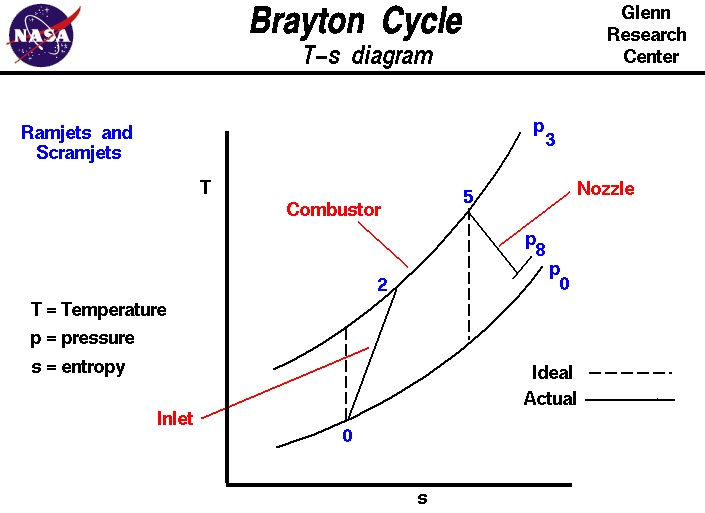
\includegraphics[width=\textwidth]{Graphics/brayton.png}
\end{minipage}
\begin{minipage}{0.48\textwidth}
	\begin{enumerate}
	\item Isentropic compression
	\item Isobaric heat addition
	\item Isentropic expansion
	\item Isobaric heat removal
	\end{enumerate}
\end{minipage}
\Item{Property Profiles}\\

\begin{minipage}{0.48\textwidth}
	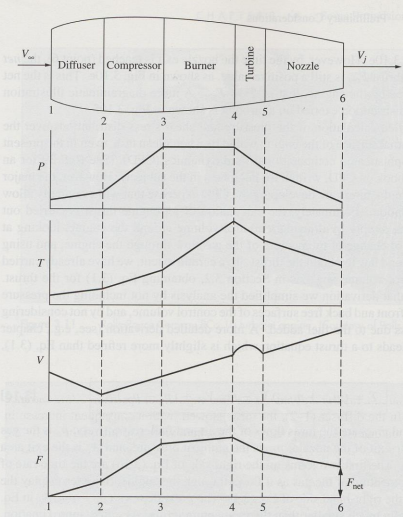
\includegraphics[width=\textwidth]{Graphics/engine_profiles.png}
\end{minipage}
\begin{minipage}{0.48\textwidth}
	\begin{itemize}
	\item Pressure increases inside the diffuser and compressor, is level through the combustor, then drops through the turbine and nozzle
	\item Temperature increases through the diffuser, compressor, and combustor, then drops through the nozzle and turbine
	\item Velocity decreases in the diffuser, then increases through the compressor and combustor, bumps up then drops through the turbine, and finally increases through the nozzle
	\item A small amount of thrust is generated by the diffuser while the bulk of the thrust is generated by the compressor. The combustor contributes a small amount while the turbine and nozzle generate forces in the drag direction
	\end{itemize}
\end{minipage}
\end{itemize}
\vspace{1cm}

\Header{Turbofans}\\
\begin{itemize}
\Item{Turbofan Terminology}
	\begin{itemize}
	\Item{Bypass Ratio} The ratio of cold air (air around core) to hot air (air through core)
	\Item{Fan Pressure Ratio} Ratio of stagnation pressure before and after the fan
	\Item{Pressure Recovery} Percent of pressure which is retained for useful work. Inlet pressure recovery typically around 90\% while burner pressure recovery is closer to 95\%, though the pressure in the burner is much higher so the losses are greater in magnitude
	\end{itemize}
\Item{Variations for High BPR Turbofans}
	\begin{itemize}
	\Item{Typical Value} About 0.6 pounds per horsepower per hour (almost half that of turbojets)
	\Item{With Velocity} Thrust decreases strongly with velocity, though it is about constant for cruise conditions. TSFC increases with velocity
	\Item{With Altitude} Thrust decreases with altitude for the same reason as turbojets (lower density). TSFC is approximately constant with altitude
	\end{itemize}
\Item{Variations for Low BPR Turbofans}
	\begin{itemize}
	\Item{Typical Value} Closely resembles turbojets, so expect 0.8-0.9 pounds per horsepower per hour
	\Item{With Velocity} Both thrust and TSFC increase with speed
	\Item{With Altitude} Thrust decreases, TSFC approximately constant
	\end{itemize}
\end{itemize}

\Header{Turboprops}\\

Turbine-driven propeller generates more thrust than a reciprocating engine/propeller combination, though less than a turbofan or turbojet. Consumes more fuel than reciprocating engine but less than turbofan or turbojet. Limited to speeds less than critical Mach number for propeller tips.

Turboprops are typically power rated rather than thrust rated. The power output is given by
\CenteredBoxed{P_A=\eta_{pr}P_S+T_j\Vinfty}
where $\eta_{pr}$ is the propeller efficiency, $P_S$ is the shaft power delivered by the engine, and $T_j$ is the thrust provided by the jet. The effective shaft power can be found by dividing by the propeller efficiency
$$P_{es}=P_S+\frac{1}{\eta_{pr}}T_j\Vinfty$$

Specific fuel consumption is based on thrust because basing it on power could lead to confusion over which power term is being referred to. Thus TSFC for turboprops is
$$c_t=\frac{\dot{W}_{fuel}}{T}$$
and a typical static installed thrust conversion is 2.5 pounds per shaft horsepower. TSFC is roughly constant with both velocity and altitude.

Power available is roughly constant with free stream Mach number due to the combined effect of increasing velocity with decreasing thrust (recall $P_A=T_A\Vinfty$). Power available decreases with altitude by a power law
$$P_A=P_{A,0}\left(\frac{\rho}{\rho_0}\right)^n$$
with $n$ depending on the engine (typically around 0.7).\\

\Header{Specific Fuel Consumptions}\\

Sometimes it is useful to be able to convert specific fuel consumptions between power rated and thrust rated aircraft. This can be done as follows and is useful for quickly formulating the range equations for either type of aircraft
$$c_t = \frac{\dot{W}_{fuel}}{T},\ c = \frac{\dot{W}_{fuel}}{P}$$
$$c_t = \frac{cP}{T},\ P = \frac{1}{\eta_{pr}}T\Vinfty$$
$$c_t = \frac{c\Vinfty}{\eta_{pr}}$$

\subsubsection{Alternative Fuels}
Renewable resource for meeting demand. Currently quite expensive and not exactly drop-in compatible, but working towards it.
\subsubsection{Electronic Propulsion}
Vehicle does not shed weight throughout the mission so range and endurance take a hit. Also have to worry about energy density, recharge time, etc.

\subsection{Structures}
\subsubsection{Brittle vs Ductile Materials}
Brittles have high Youngs moduli (relatively) but break abruptly. Ductile materials yield at a certain strain and then go plastic, reaching an ultimate strength before failing.
\subsubsection{Failure and Safety}
Common failure modes include buckling (for thin walled structures) and yield. Factors of safety are applied to the yield stresses to account for manufacturing defects, environmental conditions, inherent variability, and other sources of uncertainty in the applications of materials. A typical safety factors is in the range of 1.5 to 3. There may be a different factor of safety for each expected failure more.
$$\sigma_{des} = \frac{\sigma_{fail}}{S_F}$$
The margin of safety is defined as the ratio of the failure load to the design load, less one
$$\textrm{Margin of Safety} = \frac{\sigma_{fail}}{\sigma_{des}}-1 = S_F-1$$
\subsubsection{Aircraft Loads}
\begin{minipage}{0.63\textwidth}
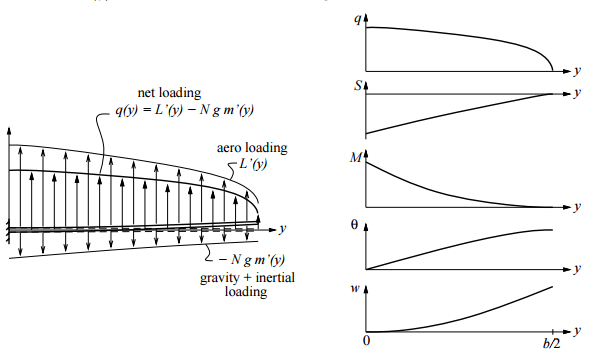
\includegraphics[width=\textwidth]{Graphics/aircraft_loads.png}
\end{minipage}
\begin{minipage}{0.35\textwidth}
$$q(y)=L'(y)-m'(y)$$
$$V(y) = V_0 + \intlim{0}{b/2}q(y)dy$$
$$V(b/2) = 0$$
$$M(y) = M_0 + \intlim{0}{b/2}V(y)dy$$
$$M(b/2) = 0 $$
\end{minipage}

Useful note from MIT document: It can be useful to assume the net distributed load is proportional to the chord distribution with the proportionality constant chosen such that the integrated loads are equal
$$q(y)=Kc(y)$$
$$\intlim{-b/2}{b/2}Kc(y)dy = \intlim{-b/2}{b/2}(L'(y)-m'(y))dy$$
$$KS_W = L-m_{wing}$$
$$K = \frac{L-m_{wing}}{S_W} \approx \frac{m_{fuselage}}{S_W}$$
\subsubsection{V-n Diagram}

\subsection{Stability and Control}
\subsubsection{Types of Stability}
Definition: Stability is the tendency of a system to maintain or deviate from an initial, established condition.
Definition: Control is the ability of a system to move between states/conditions at will
\begin{itemize}
\Item{Stable} A system is stable if any small perturbations from an equilibrium state die out with time, restoring the system to the equilibrium state
\Item{Unstable} A system is unstable if any small perturbations from an equilibrium state oscillates around or diverges from the equilibrium state
\Item{Neutral Stability} A system is neutrally stable if disturbances neither grow nor die out with time (e.g. perfect harmonic motion)
\Item{Static Stability} A system is statically stable if its initial response to a disturbance pushes it back towards its initial state (over damped stability)
\Item{Dynamic Stability} A system is dynamically stable if disturbances oscillate about the equilibrium state but decay in magnitude with time (under damped stability). Most dynamically stable systems are also statically stable (i.e. the initial response is back towards equilibrium, it just overshoots and comes back repeatedly)
\end{itemize}

A ball in a valley is stable, a ball on top of a hill is unstable. A frictionless pendulum is statically stable and dynamically neutral; a pendulum with friction is statically and dynamically stable; an inverted pendulum is statically unstable (can't even talk about dynamic properties for this case).
\subsubsection{Stability Derivatives}
Stability is often described in terms of coefficients, much like lift, drag, and moment. The coefficients in this case are the roll, pitch, and yaw moments
$$C_l = \frac{L}{qSb}$$
$$C_m = \frac{M}{qS\bar{c}}$$
$$C_n = \frac{N}{qSb}$$
Note that wing span is used as the reference length for the roll and yaw moments while mean aerodynamic chord is used for the pitching moment. The stability derivatives are taken with respect to the relevant angles, and their sign is important in talking about vehicle stability.

\subsubsection{Static Margin}

\subsection{Other Considerations}
\subsubsection{Subsystem Integration}
\subsubsection{Aircraft Economics}
\subsubsection{Life Cycle Cost Analysis}

%%%%%%%%%%%%%%%%%%%%%%%%%%%%%%%%%%%%%%%%%%%%%%%%%%%%%%

\section{Optimization}
\subsection{Standard Form of an Optimization Problem}
$$\mathrm{Minimize}\ f(\boldx)$$
$$\mathrm{w.r.t.}\ \boldx=[x_1,x_2,\dots,x_n]$$
$$s.t.\ g_j(\boldx)\leq0\ \forall j\in\mathbb{J},\ h_k(\boldx)=0\ \forall k\in\mathbb{K}$$
$$\boldx_l\leq\boldx\leq\boldx_u$$

For maximization, simply negate the objective function $f'(\boldx)=-f(\boldx)$

\subsection{Conditions for Optimality}
\subsubsection{First Order Necessary}
\begin{itemize}
\Item{Karush-Kuhn-Tucker Conditions} If a point $\xstar$ is optimal then the following hold
	\begin{enumerate}
	\item $\xstar$ is feasible
	\item $\lambda_jg_j(\xstar)=0\ \forall j\in\mathbb{J}$ (complimentary slackness)
	\item $\nabla\mathcal{L}(\xstar,\lambda)=\nabla f(\xstar)+\sumlim{j=1}{m}\lambda_j\nabla g_j(\xstar)+\sumlim{k=m+1}{\mathcal{N}}\lambda_kh_{(k-m)}(\xstar)=0,\ \lambda_i\geq0\ \forall i\in[1,\mathcal{N}]$
	\end{enumerate}
\item There are no first order \emph{sufficient} conditions for optimality. That is, there are no conditions such that a point $\xstar$ which satisfies those conditions is guaranteed to be an optimum.
\Item{Strong vs Weak Optima} An optimum $\xstar$ is a strong optimum if
\CenteredBoxed{\xstar<\boldx\ \forall \boldx\in[\xstar-\varepsilon,\xstar+\varepsilon]}
An optimum $\xstar$ is a weak optimum if
\CenteredBoxed{\xstar\leq \boldx\ \forall \boldx\in[\xstar-\varepsilon,\xstar+\varepsilon]}
\end{itemize}
\subsubsection{Second Order Necessary and Sufficient}
\begin{itemize}
\Item{The Hessian} Defined as
\[H\left(f(x_1,x_2,\dots,x_n)\right) =  \begin{bmatrix}
\PPartial{f}{x_1} & \PPPartial{f}{x_1}{x_2} & \dots & \PPPartial{f}{x_1}{x_n}\\
\PPPartial{f}{x_2}{x_1} & \PPartial{f}{x_2} & \dots & \PPPartial{f}{x_2}{x_n}\\
\vdots & \vdots & \ddots & \vdots\\
\PPPartial{f}{x_n}{x_1} & \PPPartial{f}{x_n}{x_2} & \dots & \PPartial{f}{x_n}
\end{bmatrix}\]
\Item{Necessary Conditions for Optimality} Same as first order necessary
\Item{Sufficient Conditions for Optimality} A point $\xstar$ is a global optimum if the Hessian of $f$ at $\xstar$ is positive definite (all eigenvalues are positive). A point $\xstar$ is a local optimum if the Hessian of $f$ at $\xstar$ is positive semidefinite (all eigenvalues are non-negative). These assume the goal of optimization is minimization.
\Item{Eigenvalues of the Hessian} The eigenvalues of the Hessian $\lambda_e$ are found by taking the determinant of $\Hessian(f)-\lambda_e\mathbb{I}$ and solving the resulting polynomial for $\lambda_e$

\end{itemize}

\subsection{Line Searches}
\subsubsection{Golden Section Method}
\begin{itemize}
\Item{Purpose} The Golden Section Method (GSM) is a line search technique which iteratively reduces the searchable space which brackets a minimum. The same proportional of the searchable space is thrown out with each iteration until convergence is achieved. W.L.O.G. assume $f$ is a function of only one variable.
\Item{Bracketing a Minimum} Three function values $f_1$, $f_2$, and $f_3$, evaluated at $x_1$, $x_2$, and $x_3$, respectively, with $x_1<x_2<x_3$, bracket a minimum if $f_2<f_1$ \emph{and} $f_2<f_3$. There are no guarantees about the strength of the bracketed minimum.
\Item{Steps in GSM}
	\begin{enumerate}
	\item Bracket a minimum
	\item Evaluate four points within the bracketed space: the two end points, $x_l$ and $x_u$, and two in between, $x_1$ and $x_2$
	\item Determine which endpoint to toss based on bracketing criteria. That is, determine if $\{x_l,x_1,x_2\}$ brackets the min or if $\{x_1,x_2,x_u\}$ brackets the min. Toss the end point which is not in the set which brackets the min
	\item Reassign the endpoints and generate a fourth point inside the bracket
	\item Repeat steps 3 and 4 until the desired tolerance is reached
	\end{enumerate}
\Item{Picking the New Point} The new point in the bracketed space is determined by the Golden Ratio (hence the name). This is motivated by the desire to reduce the bracketed space by the same proportion at each iteration (this is desirable because it ensures a consistent spacing of the points). The proportion is derived, from the below figure, as follows:
\begin{figure}[h]\centering
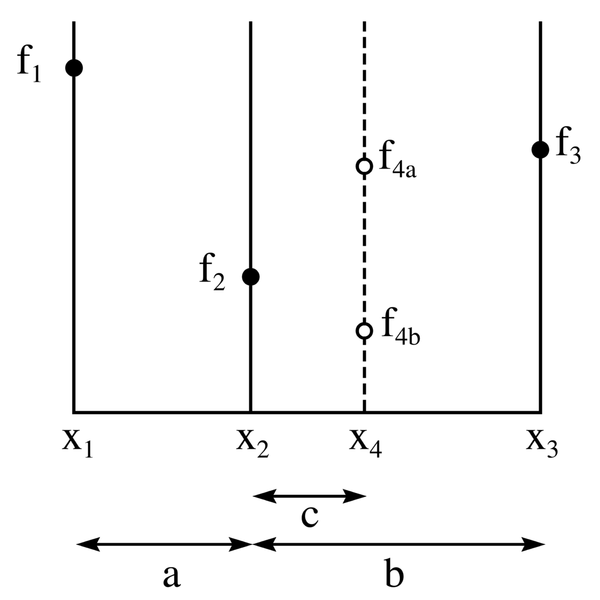
\includegraphics[scale=0.2]{Graphics/GSM.png}
\end{figure}
$$\textrm{We want } \frac{c}{a}=\frac{a}{b}\textrm{ (i.e. same proportion eliminated each time), and } c=b-a$$
$$\frac{b-a}{a}=\frac{a}{b}\to\frac{b}{a}-1=\frac{a}{b}$$
$$\frac{b}{a}\left(\frac{b}{a}-1=\frac{a}{b}\right)\to\left(\frac{b}{a}\right)^2-\frac{b}{a}-1=0$$
$$\frac{b}{a}=\frac{1\pm\sqrt{1-4(1)(-1)}}{2}=\frac{1\pm\sqrt{5}}{2}$$
\CenteredBoxed{\frac{b}{a}=1.618}
\indent The negative root was tossed for obvious reasons
\end{itemize}
\subsubsection{Direction Finding}
\subsubsection{Finding $\alpha^*$}
The methods here are of concern when a GSM is not being used. They are relevant for methods where the algorithm seeks to advance a reasonable distance along a direction, and determining what that distance should be.
\begin{itemize}
\Item{The Wolfe Conditions} The Wolfe conditions are two conditions which can be used to determine the step size along a given direction. They come in strong and weak forms. The weak form is to find $\alpha$ such that the following hold
	\begin{enumerate}
	\item Armijo: $\boxed{f(\boldx_{k-1}+\alpha\mathbf{s}_k)\leq f(\boldx_{k-1})+c_1\alpha\mathbf{s}_k^T\nabla f(\boldx_{k-1}}$. This rule requires the function to not change too much along the given search direction. The ''too much'' conditional is expressed through the constant $c_1\in[0,1]$ and typically $c_2\approx 10^{-4}$, and the gradient of the function (higher gradients allow for larger step sizes)
	\item Curvature: $\boxed{\mathbf{s}_k^Tf(\boldx_{k-1}+\alpha\mathbf{s}_{k-1})\geq c_2\mathbf{s}_k^T\nabla f(\boldx_{k-1})}$. This condition requires the step size to be large enough that the gradient changes meaningfully. The `'meaningful'' conditional is expressed through the constant $c_2\in[0,1]$ and typically $c_2\approx0.9$. Note that gradients will be negative in the search direction (assuming minimization) so the gradient should become \emph{less negative}
	\end{enumerate}
	
	The strong form is to find $\alpha$ such that the following hold
	\begin{enumerate}
	\item Armijo: $\boxed{f(\boldx_{k-1}+\alpha\mathbf{s}_k)\leq f(\boldx_{k-1})+c_1\alpha\mathbf{s}_k^T\nabla f(\boldx_{k-1}}$. Unchanged from weak conditions
	\item Curvature: $\boxed{|\mathbf{s}_k^Tf(\boldx_{k-1}+\alpha\mathbf{s}_{k-1})|\leq c_2|\mathbf{s}_k^T\nabla f(\boldx_{k-1})|}$. Now we require that the \emph{magnitude} of the gradient decrease by a meaningful amount 
	\end{enumerate}
\end{itemize}

\subsection{Indirect Methods for Constrained Optimization}
Indirect methods provide means to incorporate constraints into the optimization formulation. They work by augmenting the initial objective function such that the new pseudo-objective function can be minimized in an unconstrained way (e.g. line search). They may, however, provide suboptimal or infeasible results if proper care is not taken in their formulation.
\subsubsection{Exterior Penalty Method}
Perhaps the simplest of the indirect methods, the exterior penalty method adds the constraint value to the objective value when the constraint is active. That is, the augmented objective function becomes
\CenteredBoxed{\Phi(\boldx,r_p)=f(\boldx) + r_p\left[ \sumlim{j=1}{l}\max[0,g_j(\boldx)]^2 + \sumlim{k=1}{m}[h_{k}]^2\right]}
where the variable $r_p$ scales the penalty for violating any of the constraints. Typically, $r_p$ will start small and increase as the optimization procedure goes on.

The exterior penalty method has a tendency to allow infeasible designs. The penalty may not be able to overcome the gradient of the objective at the boundary if the gradient is steep enough, and thus may require $r_p\to\infty$, which is impractical. The function also becomes extremely nonlinear at the boundaries which could cause problems for line searches. It is, however, extremely simple to implement.

\subsubsection{Interior Penalty Method}
The interior penalty method only applies to inequality constraints (equality constraints have no interior). The method imposes a penalty for getting close the constraint boundaries, then relaxes those penalties as the procedure advances. This formulation allows the optimizer to approach the optimum from within the feasible space. It may, however, yield suboptimal results if the procedure is terminated early. The augmented objective function becomes
\CenteredBoxed{\Phi(\boldx,r_p,r_p')=f(\boldx) + r_p'\sumlim{j=1}{l}\frac{-1}{g_j(\boldx)} + r_p\sumlim{k=1}{m}[h_{k}]^2}
where $r_p'$ is a new penalty factor which starts very large and decreases (to one) as the optimization procedure advances. An alternative formulation uses the logarithm of the inequality constraints, becoming
\CenteredBoxed{\Phi(\boldx,r_p,r_p')=f(\boldx) + r_p'\sumlim{j=1}{l}-\log[-g_j(\boldx)] + r_p\sumlim{k=1}{m}[h_{k}]^2}

\subsubsection{Extended Interior Penalty Method}
Similar to the standard interior penalty method but with a modification to enable finding truly optimal points. Each inequality constraint is modified such that
\[\tilde{g}_j(\boldx)=\begin{cases}
\frac{-1}{g_j(\boldx)} & g_j(\boldx)\leq\varepsilon\\
-\frac{2\varepsilon-g_j(\boldx)}{\varepsilon^2} & g_j(\boldx)>\varepsilon
\end{cases}\]
with $\varepsilon = -c(r_p')^a$, $-1/3\leq a\leq1/2$ and $c=const.$. This linearizes the constraint near the boundary on the feasible side

\subsubsection{Constraint Scaling}
Constraints can be scaled to the order of the objective function. This is done to aid smoothness of the pseudo-objective, which in turn helps whatever methods are chosen for finding the optimum. Constraints should be scaled according to
$$\bar{g}_j(\boldx)=c_jg_j(\boldx)$$
$$c_j=\frac{|\nabla f(\boldx)|}{|\nabla g_j(\boldx)|}$$
With these scalings, the initial values for the penalty factors $r_p$ and $r_p'$ are one.

\subsubsection{The Augmented Lagrangian}
The Augmented Lagrangian combines Lagrange's method of undetermined coefficients with the exterior penalty method to come up with a new pseudo-objective function. The ALM pseudo-objective is given by
$$\mathbf{A}(\boldx,\lambda,r_p)=\mathcal{L}(\boldx,\lambda) + r_p\left[\sumlim{j=1}{l}g_j(\boldx)^2 + \sumlim{k=1}{m}\left(h_k(\boldx)\right)^2\right]$$
\CenteredBoxed{\mathbf{A}(\boldx,\lambda_p,r_p) = f(\boldx) + \sumlim{j=1}{l}\left[\lambda_j\psi_j(\boldx) + r_p\left[\psi_j(\boldx)\right]^2\right] + \sumlim{k=1}{m}\left[\lambda_{p,k+m}h_k(\boldx) + r_p[h_k(\boldx)]^2\right]}
where
$$\psi_j(\boldx)=\max\left[g_j(\boldx),\frac{-\lambda_{p,j}}{2r_p}\right]$$
The augmented Lagrangian is derived from a comparison of the standard Lagrangian and the exterior penalty methods, as follows.
\begin{itemize}
\item Consider a potential optimal point $\xstar$. At this point, the following must hold
$$\nabla\mathcal{L}(\xstar,\lambda) = \nabla f(\xstar) + \sumlim{\textrm{active}}{}\lambda_j\nabla g_j(\xstar) + \sum\lambda_k\nabla h_k(\xstar) = 0$$
$$\nabla\Phi(\xstar,r_p) = \nabla f(\xstar) + r_p\left[\sumlim{\textrm{active}}{}2g_j(\xstar)\nabla g_j(\xstar) + \sum2h_k(\xstar)\nabla h_k(\xstar)\right] = 0$$
\item Equating these two equations and comparing the coefficients of the derivatives yields
$$2r_pg_j(\xstar)=\lambda_j,\quad 2r_ph_k(\xstar)=\lambda_k$$
which, after rearranging and applying complimentary slackness from the KKT conditions, reveals that we require $r_p\to\infty$
\item We can get around the $r_p\to\infty$ problem by realizing the gradient augmented Lagrangian must go to zero along with that of the true Lagrangian itself. That is,
$$\nabla\mathbf{A}(\xstar,\lambda_p,r_p)=\nabla\mathcal{L}(\xstar,\lambda)=0$$
\item After applying the gradients and simplifying, we arrive at the following
$$\lambda_j=\lambda_{p,j}+2r_p\max\left[g_j,\frac{-\lambda_{p,j}}{2r_p}\right]$$
$$\lambda_k=\lambda_{p,k}+2r_ph_k(\xstar)$$
These formulas can be used to update the Lagrange multiplier estimates at each iteration while maintaining complimentary slackness and being relatively insensitive to choices in $r_p$
\item A note on Lagrange multipliers: They can be roughly interpreted as the cost of having that constraint be there. Consider a function with one constraint evaluated at the optimum point where that constraint is active. Then the following holds
$$\nabla f(\xstar)+\lambda\nabla g(\xstar)=0$$
$$\lambda=\frac{-\nabla f(\xstar)}{\nabla g(\xstar)}$$
Thus $\lambda$ can be interpreted as the ratio of the improvement in $f$ to the degradation of $g$. High Lagrange multipliers imply significant improvement may be made in the objective function by relaxing that constraint, relative to the penalty incurred by that constraint. Complimentary slackness tells us there is no benefit to relaxing an inactive constraint.
\end{itemize}

\subsection{Zeroth Order Methods}
\subsubsection{Random Search}
Take a step in a random direction from an initial point. If that new point is better than the current point then go there, otherwise find a new random point. Repeat.
\subsubsection{Grid Search}
Discretize the design space and evaluate the objective function at nodes (where grid lines cross), then take the best one
\subsubsection{Compass Search}
From a starting location sample a $\pm1$ unit step in each design variable independently. Move to the point which provides the best improvement over the current point. Repeat at new point (obviously not re-sampling the point you just came from).
\subsubsection{Univariate Search}
Perform the GSM algorithm along each design variable independently and iteratively (i.e. GSM along $x_1$, then $x_2$, and so on to $x_n$, then repeat).
\subsubsection{Powell's Method}
\begin{itemize}
\Item{Overview} Apply conjugacy condition to univariate search algorithm to improve convergence behavior
\Item{Method}
	\begin{enumerate}
	\item Do one pass over the univariate search method (i.e. do GSM in each univariate direction)
	\item Determine the $(n+1)^{th}$ search direction such that is is conjugate to all other directions
	\item Definition of conjugacy: Two vectors $\mathbf{s}_i$ and $\mathbf{s}_j$ are conjugate w.r.t. a matrix $\mathbb{A}$ if
	$$\mathbf{s}_i'\mathbb{A}\mathbf{s}_j=0$$
	in the case of Powell's method $\mathbb{A}=\mathbb{I}$ and $\mathbf{s}_{n+1}=\sumlim{i=1}{n}\alpha_i\mathbf{s}_i$ where $\mathbf{s}_i$ are unit vectors and $\alpha_i$ is the distance between the initial and final points for the $i^{th}$ search direction. The $(n+1)^{th}$ search direction is simply the (normalized) weighted sum of the previous $n$ search directions, with the step size as the weighting criteria
	\end{enumerate}
\Item{Benefits} For a quadratic problem with $n$ variables, convergence will be achieved in at most $n$ cycles
\Item{Drawbacks} Search directions tend to coalesce as the algorithm gets into its later stages (requires resetting search directions to univariates)
\end{itemize}

\subsection{First Order Methods}
First order methods are mostly concerned with determining the search direction from derivative information and performing line searches in those directions.
\subsubsection{Steepest Descent}
\begin{itemize}
\Item{Definition} Steepest descent picks the search direction which provides the most rapid improvement in the objective function. That is, the search direction is found to be
\CenteredBoxed{\mathbf{s}_k=\frac{-\nabla f(\boldx_{k-1})}{\|f(\boldx_{k-1})\|}}
\end{itemize}
\subsubsection{Fletcher-Reeves Conjugate Gradient}
The Fletcher-Reeves method applies conjugacy to the gradient of the objective function at each point, analogous to how Powell's applied conjugacy to directions. The new search direction is found via the update method
\CenteredBoxed{\mathbf{s}_{k+1}=-\nabla f_{k}+\beta_k\mathbf{s}_{k}}
$$\beta_k=\frac{\|\nabla f_{k}\|^2}{\|\nabla f_{k-1}\|^2}$$

Fletcher-Reeves modifies the steepest descent direction with derivative information from previous steps. The first direction will be the steepest descent direction
\subsubsection{Broyden-Fletcher-Goldfarb-Shanno Quasi-Newton Method}
BFGS uses an approximation of the Hessian matrix to find the search direction. The Hessian is approximated by applying a finite difference to gradient information and updating the approximation as the algorithm proceeds. The method finds the search direction as
\CenteredBoxed{\mathbf{s}_{k+1}=-B_k\nabla f(\boldx_k)}
where
\CenteredBoxed{B_{k+1}=B_k+\frac{(\Delta(\nabla f_{k,k-1})-B_k\Delta\boldx_{k,k-1})(\Delta(\nabla f_{k,k-1})-B_k\Delta\boldx_{k,k-1})^T}{(\Delta(\nabla f_{k,k-1})-B_k\Delta\boldx_{k,k-1})^T\Delta\boldx_{k,k-1}}}
and $B_0=\mathbb{I}$ (i.e. first direction is steepest descent)
\subsection{Second Order Methods}
\subsubsection{Newton's Method}
Newton's method finds the next search direction by inclusion of Hessian (second order) information. The search direction is found via
\CenteredBoxed{\mathbf{s}_{k+1}=-\left[H(\boldx_k)\right]^{-1}\nabla f(\boldx_k)}
\begin{itemize}
\Item{Benefits} If the function is quadratic then Newton's method will find the optimum in one step
\Item{Drawbacks} The inverse of the Hessian may not exist (if it is not positive definite) and can be computationally expensive if it is. BFGS is one way to work around this
\end{itemize}

\subsection{Multi-Objective Optimization}
\subsubsection{Domination Criteria and Pareto Optimality}
Optimality is more difficult for multi-objective problems because of the comparability problem. It would be impossible to compare two designs unless we were able to apply a strict preference to the set of objectives. One way around this is Pareto analysis, in which the set of best designs is separated from the rest of the space. The Pareto optimal set consists of all nondominated designs, either strongly or weakly so. A design is said to be strongly nondominated if there exists no other design whose objective values are strictly better than its own. That is, assuming minimization is the objective,
$$\xstar\in\mathbb{P}\iff f(\xstar)<f(\boldx)\ \forall\boldx\in\mathbb{D}\ \&\ \forall f\in\mathbb{F}$$
Weak domination removes the strictness of the inequality
$$\xstar\in\mathbb{P}\iff f(\xstar)\leq f(\boldx)\ \forall\boldx\in\mathbb{D}\ \&\ \forall f\in\mathbb{F}$$

\subsubsection{Finding the Pareto Frontier}
\begin{itemize}
\Item{Weighted Sum Approach} Consolidate the multiple objective functions into a single objective which is a weighted sum of all the objectives. Changing the weighting scheme changes where on the Pareto front the algorithm will converge. Benefits: Easy. Drawbacks: Cannot sample convex spaces
\Item{Epsilon-Constraint Method} The epsilon-constraint method reduces the multi-objective problem to a single objective problem by converting the other objective(s) into constraints. The optimizer will then seek to optimize a the free objective while keeping the other(s) below a given margin. This is best visualized with a two-objective minimization problem
\Item{Normal Boundary Intersection} Designed to evenly sample the Pareto frontier. For a 2D problem this method draws a line between the best points in each objective dimension, then moved in the normal direction to that line (in the improvement direction, of course) until the optima along that line are found. This can be thought of as minimizing $f_1$ subject to $f_2=\alpha+\beta f_1$
\end{itemize}

\subsection{Metaheuristic Methods}
\subsubsection{Particle Swarm}
Based loosely on swarm animal/insect behaviors, each design point moves according to some rules so as to improve its own objective value. Particles may interact with neighbors or entire swarm. Velocity update may include inertia (history), local best, global best, pushoff factors, or other terms.
\subsubsection{Simulated Annealing}
Based on the idea of a cooling piece of metal and the minimization of energy within the crystalline structure. A cooling schedule governs the likelihood of accepting a new point with a worse objective value, while points with better objective values are always taken. Probability of accepting a new point $\xstar$ from a starting point $\boldx$ given by decaying exponential
$$P(\boldx,\textrm{accept }\xstar) = \min\left[e^{-\Delta E/kT_i},1\right]$$
$$\Delta E = f(\xstar)-f(\boldx)$$
$$T_i=\gamma T_{i-1},\ \gamma<1$$
Clearly if $\Delta E$ is negative ($f(\boldx)>f(\xstar)$) then the probability is greater than one. The decrease of $T$ with each iteration makes the exponent more negative for the same $\Delta E$, meaning worse candidate points are less likely to be accepted.
\subsubsection{Genetic Algorithm}
The genetic algorithm takes inspiration from biology. Design variable vectors are converted to chromosomes with each gene representing a single design variable. The objective function values determine the fitness of an individual. Crossover and mutation provide the means for exploitation and exploration, respectively. The NSGA-II uses Pareto frontier information to select the best candidates at each generation, which then carry over to the next generation.

GAs require the design variables to be discretized. This can give rise to issues with extremely long chromosomes resulting from very fine resolutions or missing large parts of the design space because the discretization is too coarse. The number of bits required for a given range and resolution on a design variable is given by
$$N\geq\log_2\left(\frac{Range}{Resolution}+1\right)$$

Gray coding can be used to avoid the Hamming cliff problem. The Hamming cliff problem arises from binary representations because the number of bits which must flip to increment a variable by one unit may be extremely large. For example, turning 7 (0111) into 8 (1000) requires flipping all four bits. Gray coding operates on pairs of bits. The first bit is retained and each successive bit is set to 0 if the corresponding and previous bits of the original string are the same, and 1 otherwise. For example, 0111 converted to gray code would be 0100 while 1000 would be 1100. Thus the number of bits which must flip to increment 7 to 8 is just one. In most practical applications with large population sizes gray coding is unnecessary.

\subsection{Surrogate Modeling}
\subsubsection{Polynomial Basis Functions}
\begin{itemize}
\Item{Purpose} Rather than sampling the true function we can create a model representation of the function and attempt to minimize that, then check our result with the true function to ensure accuracy
\Item{Method}
	\begin{enumerate}
	\item Sample the design space with a DOE
	\item Fit or train the models, determining the parameters in the approximation function to best match the true function
	\item Validate the fitted approximation function with data not used for training to ensure the model is good
	\item Predict new values using the new function and perform optimization on that
	\end{enumerate}
\Item{Theory} A surrogate model can be represented in the form
$$\hat{f}(\boldx_j)=\sumlim{i}{n}w_i\phi_i(\boldx_j)$$
This formulation leads to the following
$$f(\boldx_j) = \hat{f}(\boldx_j) + \varepsilon(\boldx_j) = \sumlim{i}{n}w_i\phi_i(\boldx_j) + \varepsilon(\boldx_j)$$
With $f$, $w_i$ and $\phi_i$ known, the error is found by
$$\varepsilon(\boldx_j)=f(\boldx_j)-\sumlim{i}{n}w_i\phi_i(\boldx_i)$$
$$\bm{\varepsilon}=\bm{f}-\Phi\bm{w}$$
A good model will have low error -- really a low norm-squared error -- which can be represented by the least squares problem
$$\min\bm{\varepsilon}^T\bm{\varepsilon}\ \mathrm{w.r.t.}\ \bm{w}$$
The solution to this problem is analytic given the above formulation, as follows
$$\frac{d}{d\bm{w}}\bm{\varepsilon}^T\bm{\varepsilon} = 2\left(\frac{d\bm{\varepsilon}}{d\bm{w}}\right)^T\bm{\varepsilon}=0$$
$$\bm{\varepsilon}=\bm{f}-\Phi\bm{w}\implies \frac{d\bm{\varepsilon}}{d\bm{w}}=-\Phi$$
$$\Phi^T(\bm{f}-\Phi\bm{w})=0$$
\CenteredBoxed{\bm{w}=\left(\Phi^T\Phi\right)^{-1}\Phi^T\bm{f}}
\Item{Approximation Functions} Polynomials are a common choice. A high number of variables (high dimensionality of the design space) with a high degree may require a significant number of terms, which may make the model difficult to train. For example, with two variables and two levels (i.e. maximum exponent is 2) there are five possible terms: 1, $x_1$, $x_2$, $x_1x_2$, $x_1^2$, $x_2^2$. For eight variables at eight levels there are 12870 possible terms. The general formula is given below, where $q$ is the order, up to $n$, and $p$ the number variables.
\CenteredBoxed{\mathcal{N}_{terms} = \sumlim{q=1}{n}{{q+p-1}\choose{q}} = \sumlim{q=1}{n}\frac{(q+p-1)!}{(q!)(p-1)!}}
\Item{Number of Training Points for Fitting} Let $\bm{f}$ and $\bm{\varepsilon}$ be $m$-element vectors, $\bm{w}$ and $n$-element vector, and $\Phi$ an $m\times n$ matrix. Then the three following cases are possible
	\begin{enumerate}
	\item $m<n$: less training points than basis functions $\to$ model is underdetermined ($\Phi^T\Phi$ is singular and model cannot be fit)
	\item $m=n$: as many training points as basis functions $\to$ model is perfectly determined (interpolant)
	\item $m>n$: more training points than basis functions $\to$ model is overdetermined (least squares)
	\end{enumerate}
For a polynomial basis of one variable up to degree $n$ with $m$ training points, the $\Phi$ matrix will look like
$$\phi_{i,j}=x_j^i,\ i\in[0,n],\ j\in[1,m]$$
\[\Phi(\boldx) =  \begin{bmatrix}
x_1^0 & \dots & x_1^{n}\\
\vdots & \ddots & \vdots\\
x_m^0 & \dots & x_m^n\\
\end{bmatrix}\]

Adding more basis functions is not necessarily a good thing. Model overfitting can occur, where the model starts overshooting the actual function -- particularly near the edges of the domain -- as a result of having higher order terms. In general, there is no way to predict if/when overfitting will start or stop being a problem. Thus it is usually a better idea to fit a relatively simple basis to a large set of training data.
\Item{Quality of Fits} The sum squared error and squared residual (coefficient of determination) are common methods for checking model error. The sum squared error is given by 
$$SSE=\bm{\varepsilon}^T\bm{\varepsilon}=(\bm{y}-\bm{\hat{y}})^T(\bm{y}-\bm{\hat{y}})$$
where $\bm{y}$ are the observed function values and $\bm{\hat{y}}$ are the predicted function values, both taken at the training points. The coefficient of determination is given by
$$R^2=1-\frac{SSE}{SST},\ SST=(\bm{y}-\bm{\bar{y}})^T(\bm{y}-\bm{\bar{y}})$$
where $\bm{\bar{y}}$ is the mean of the observed function values at the training points. The sum squared error should be low (it will be zero for an interpolating model) and the residual should be correspondingly close to 1.\\

Validation is also an important step in assessing models. Validation takes place at data points which were \emph{not} used to train the data. The sum squared error and coefficient of determination are calcuated in the same way as before, with the same criteria for goodness of fits. Note that validation errors will (probably) not be zero even for interpolating models.
\Item{Regularization or Ridge Regression} It may be the case that a higher order polynomial -- at least in the case of polynomial basis functions -- are desired such that $n>m$, or if there are basis functions which are known to be insignificant to the true function. In this case, the least squares problem is modified to encourage minimization of the norm of the weights
$$\min\left(\bm{\varepsilon}^T\bm{\varepsilon} + \lambda\bm{w}^T\bm{w}\right)\ \mathrm{w.r.t.}\ \bm{w}$$
where $\lambda>0$ is called the ridge parameter and is set a priori to control which effect is dominant. Carrying out the same procedure as before, we arrive at the following expression for the weights
\CenteredBoxed{\bm{w}=\left(\Phi^T\Phi+\lambda\mathbb{I}\right)^{-1}\Phi^T\bm{f}}
This matrix is \emph{always} invertible, and so the result is not rank deficient and the model can be created. This approach tends to spread out the effect of the true parameters, though the effects spread to nearby parameters (i.e. a linear dependence may ``bleed'' over to the quadratic basis).
\end{itemize}
\subsubsection{Radial Basis Functions}
\begin{itemize}
\Item{Theory} Essentially the same as polynomial basis, just that the basis function is based on proximity to training data. That is,
\CenteredBoxed{\hat{f}(\boldx_j)=\sumlim{i}{n}w_i\phi(\|\boldx_j-\boldx_i\|)}
Note that there is only one basis function in this equation. More precisely, there only one \emph{form} of the basis function for RBFs.
\Item{Choosing a Radial Basis} In practice, the choice of radial basis function is largely irrelevant. A few common choices are
	\begin{align}
	\textrm{Multiquadric: }\phi(r)&=\left(r^2+r_0^2\right)^{1/2}\\
	\textrm{Inverse Multiquadric: }\phi(r)&=\left(r^2+r_0^2\right)^{-1/2}\\
	\textrm{Thin Plate Spline: }\phi(r)&=r^2\ln\left(\frac{r}{r_0}\right)\\
	\textrm{Gaussian: }\phi(r)&=\exp\left(\frac{-r^2}{2r_0^2}\right)\\
	\textrm{Cubic: }\phi(r)&=1+\frac{r^3}{r_0^3}
	\end{align}
\Item{Fitting a Radial Basis} RBFs are typically implemented as interpolating functions ($m=n$), so $\Phi$ is square, symmetric, and invertible
$$\phi_{i,j}=\phi(\|\boldx_j-\boldx_i\|)=\phi(\|\boldx_i-\boldx_j\|)=\phi_{j,i}$$
\[\Phi(\boldx) =  \begin{bmatrix}
\phi(\|\boldx_1-\boldx_1\|) & \dots & \phi(\|\boldx_1-\boldx_n\|)\\
\vdots & \ddots & \vdots\\
\phi(\|\boldx_n-\boldx_1\|) & \dots & \phi(\|\boldx_n-\boldx_n\|)\\
\end{bmatrix}\]
The following are direct consequences of this
$$(\Phi^T\Phi)^{-1}\Phi^T=\left[\Phi^{-1}(\Phi^T)^{-1}\right]\Phi^T=\Phi^{-1}$$
$$\bm{w}=\Phi^{-1}\bm{f}$$
$$\bm{\varepsilon}=\bm{f}-\Phi\bm{w}=\bm{f}-\Phi\Phi^{-1}\bm{f}=0$$
\end{itemize}
\subsubsection{Artificial Neural Networks}
Artificial Neural Networks attempt to emulate synapse firing in the brain. The same functional form is used as for radial basis functions, but the argument to the activation function $\phi$ is a linear function of the $p$-element design variable vector
$$\hat{f}(\boldx)=\sumlim{i=1}{m}\alpha_i\phi(a_i),\ a_i = \sumlim{j=1}{p}w_{i,j}x_j + \beta_j = \bm{\beta} + \sumlim{j=1}{p}w_{i,j}x_j$$
where the parameters $\alpha_i$, $w_{i,j}$, and $\beta_j$ must all be found during the training process. The activation function is typically chosen to be a smooth approximation to the step function (Heaviside theta), such as the logistic curve of inverse tangent
$$\phi(a_i)=\frac{1}{1+\exp(-a_i)}$$
$$\hat{f}(\boldx) = \sumlim{i=1}{m}\frac{\alpha_i}{1+\exp\left(-\bm{\beta}-\sumlim{j=1}{p}w_{i,j}x_j\right)}$$

$$\phi(a_i)=\tan^{-1}(a_i)$$
$$\hat{f}(\boldx) = \sumlim{i=1}{m}\alpha_i\tan^{-1}\left(\bm{\beta} + \sumlim{j=1}{p}w_{i,j}x_j\right)$$

%%%%%%%%%%%%%%%%%%%%%%%%%%%%%%%%%%%%%%%%%%%%%%%%%%%%%%

\section{Thermodynamics}
\subsection{Background Mathematics}
\subsubsection{Exact Differential}
An exact differential is path independent and obeys the following rules for first and second derivatives
$$dz = \PartialConst{z}{x}{y}dx + \PartialConst{z}{y}{x}dy$$
$$\Partial{}{y}\Partial{z}{x} = \Partial{}{x}\Partial{z}{y}$$

\subsection{Classical Thermodynamics}
\subsubsection{The State Postulate}
\large\emph{The number of independent, intensive thermodynamic properties of a specified substance is equal to the number of relevant reversible work modes plus one. In the case of a simple compressible substance, two independent intensive properties are needed to completely define the thermodynamic state.}\\\normalsize

\textbf{Definition:} A simple substance is one for which there is only one reversible work mode. A simple compressible substance is one where that reversible work mode is fluid compression.

\textbf{Definition:} A reversible work mode is one where the the force is independent of direction and rate of change. The former implies the work done by a force $F$ in the direction $+dx$ is equal in magnitude to the work done by the same force in the directino $-dx$. Reversible work can be accounted for by reversible work plus heat transfer.

\subsubsection{The First Law of Thermodynamics}
\large\emph{For a closed system where $dKE=dPE=0$, there exists a state variable $U$ such that, for an infinitessimal change in state,}
\CenteredBoxed{dU=\delta Q + \delta W}
\normalsize

\subsubsection{The Second Law of Thermodynamics}
\large\emph{There exists a state variable $S$ which can be produced but cannot be destroyed}
\CenteredBoxed{S_2-S_1=\Delta S \geq 0}
\normalsize

\textbf{Thermodynamic Definition of Temperature:}
Consider an isolated system split into two parts of constant volume which may interact. The entropy of the system can be expressed as 
$$S_C=S_A(U_A,V_A) + S_B(U_B,V_B)$$
Define the variable $\mu$ to track the progress of the thermal change of the system (assuming there is any) through heat transfer. Then we have the following
$$\frac{dS_C}{d\mu}=\PartialConst{S_A}{U_A}{V_A}\Partial{U_A}{\mu} + \PartialConst{S_B}{U_B}{V_B}\Partial{U_B}{\mu}$$
We know, from the second law of thermodynamics applied to isolated systems, that $$\frac{dS_C}{d\mu}=0$$. Also, from the first law applied to isolated systems, we know $$\frac{dU_C}{d\mu}=\frac{d}{d\mu}(U_A+U_B)=0$$. Therefore,
$$\PartialConst{S_A}{U_A}{V_A}=\PartialConst{S_B}{U_B}{V_B}$$
This allows us to define thermal equilibirum as the state at which the above equality holds. Furthermore, we can define temperature as the reciprocal of the rate of change of entropy with respect to internal energy at constant volume (reciprocal used such that heat flows from high to low temperatures).
\CenteredBoxed{T=\frac{1}{\left(\partial S/\partial U\right)_{V}}}

\textbf{Thermodynamic Definition of Pressure:}
Consider the same example as before but with the addition that the parts may exchange energy in the form of $pdV$ work.  Then we can define a new tracking variable $\mu_V$ which tracks the progress of the mechanical change of the system. Then
$$\frac{dS_C}{d\mu_V}=\PartialConst{S_A}{V_A}{U_A}\Partial{V_A}{\mu_V} + \PartialConst{S_B}{V_B}{U_B}\Partial{V_B}{\mu_V}$$
$$\PartialConst{S_A}{V_A}{U_A}=\PartialConst{S_B}{V_B}{U_B}\to p = T\PartialConst{S}{V}{U}$$

\textbf{The Gibbs Equation:}
For a simple compressible nonreacting substance we have the following
$$S = S(U,V)$$
$$dS = \PartialConst{S}{U}{V}dU + \PartialConst{S}{V}{U}dV$$
which, from our previous definitions, simplifies to
$$dS = \frac{1}{T}dU + \frac{p}{T}dV$$
or
\CenteredBoxed{dU = TdS - pdV}

\textbf{Entropy and Entropy Production:}
Consider a resevoir of fixed mass which maintains a constant temperature $T_r$. Then the Gibbs equation reduces to
$$dU = T_rdS$$
Consider a differential amount of heat being added to (or taken from) the resevoir. The first law states
$$dU = \delta Q\implies dS = \frac{\delta Q}{T_r}$$
Therefore we conclude that entropy can result from the exchange of heat.

Now consider two bodies, one at $T_A$ and the other at $T_B$ with $T_A<T_B$, which exchange an amount of heat $\delta Q$ (from B to A). Then the entropy change of each body is
$$dS_A =  \frac{\delta Q}{T_A}\geq0,\quad dS_B = - \frac{\delta Q}{T_B}\leq0$$
$$dS_B = -\frac{T_A}{T_B}dS_A$$
$$dS_{A+B} = dS_A + dS_B = dS_A\left(1-\frac{T_A}{T_B}\right)\geq0$$
Thus there is entropy \emph{generation} due to heat transfer across finite temperature differences.

\subsubsection{Chemical Potential}
Previous results were obtained for a simple compressible substance of a single species. Now consider a mixture of simple compressible substances such that the entropy is a function of the two variables plus composition $S = S(U,V,n_1,n_2,...,n_k)$, and
$$dS = \PartialConst{S}{U}{V,n_i}dU + \PartialConst{S}{V}{U,n_i}dV + \sumlim{i=1}{k}\PartialConst{S}{n_i}{U,V,n_j}dn_i$$
$$dS = \frac{1}{T}dU + \frac{p}{T}dV - \sumlim{i=1}{k}\frac{\mu_i}{T}dn_i$$
Chemical potential is used to describe equilibrium of phase (or composition) in the same way temperature and pressure are used to describe thermal and mechanical equilibrium, respectively.

The chemical potential can be related to the Gibbs free energy in the following manner
$$G = G(p,T,n_i)$$
$$dG = \PartialConst{G}{p}{T,n_i}dp + \PartialConst{G}{T}{p,n_i}dT + \sumlim{i=1}{k}\PartialConst{G}{n_i}{p,T}dn_i$$
$$G = H - TS \implies dG = dH - TdS - SdT $$
$$dG = dU + pdV + Vdp - \left(dU - pdV -\sumlim{i=1}{k}\mu_idn_i\right) - SdT$$
$$dG = Vdp - SdT + \sumlim{i=1}{k}\mu_idn_i$$
Equating the seocnd and last equations above results in the following
$$\PartialConst{G}{p}{T,n+i}=V,\quad\PartialConst{G}{T}{p,n_i}=-S,\quad\PartialConst{G}{n_i}{p,T}=\mu_i$$
This leads to the important result that the chemical potential of a pure substance of a single phase is equal to its molar Gibbs free energy.

Three possible criteria for equilibrium are:
\begin{enumerate}
\Item{Constant U and V} $dS = dU + pdV - \sumlim{i=1}{k}\mu_idn_i \geq 0$
\Item{Constant T and V} $dF = -SdT - pdV + \sumlim{i=1}{k}\mu_idn_i \leq 0$
\Item{Constant T and P} $dG = Vdp - SdT + \sumlim{i=1}{k}\mu_idn_i \leq 0$
\end{enumerate}
All three of these criteria require the following for equilibrium
\CenteredBoxed{\sumlim{i=1}{k}\mu_idn_i \leq 0}
That is, minimization of the sum of chemical potentials is a general requirement for equilibrium for multicomponent systems. We can apply this to simple reactions by defining a progress variable $\eta$ and finding its value such that the chemical potential of the system is minimized. Take the sample reaction $H_2 + Cl_2 \leftrightharpoons 2HCl$.
$$d\eta = \frac{dn_i}{\nu_i}$$
$$\nu_{H_2} = -1,\ \nu_{Cl_2} = -1,\ \nu_{HCl} = +2$$ 
$$\sum\mu_idn_i=\sum\mu_i(\nu_id\eta)=d\eta\left(\sum\mu_i\nu_i\right)\leq0$$
By convention $\eta\in[0,1]$ (i.e. $\eta=0$ if the composition is entirely LHS compounds and $\eta=1$ ifthe composition is entirely RHS compounds) so we require $\sum\mu_i\nu_i\leq0$. Therefore, if $\sum\mu_i\nu_i<0$ then the reaction will proceed from left to right (i.e. more of the positive $\nu$ compounds will be formed). Otherwise, if $\sum\mu_i\nu_i>0$ then the reaction will proceed form right to left (i.e. more of the negative $\nu$ compounds will be formed). Finally, if $\sum\mu_i\nu_i=0$ then equilibrium has been achieved (i.e. neither positive nor negaitve $\nu$ compounds are favored).

\subsubsection{Maxwell's Relations}
Maxwell's relations derive from the state postulate and the rules of exact differentials. Take, for example, the internal energy of a system
$$U = U(S,V)$$
$$dU = \PartialConst{U}{S}{V}dS + \PartialConst{U}{V}{S}dS$$
$$dU = TdS - pdV$$
then the second derivative rule for exact differentials requires
$$\PartialConst{T}{V}{S} = -\PartialConst{p}{S}{V}$$
We can perform similar operations on the enthalpy, Helmholtz free energy, and Gibbs free energy and arrive a similar results (these all assume $dn_i=0$)
$$dH = dU + d(pV) = TdS + Vdp \implies \PartialConst{T}{p}{S} = \PartialConst{V}{S}{p}$$
$$dF = dU - d(ST) = -SdT - pdV \implies \PartialConst{S}{V}{T} = \PartialConst{p}{T}{V}$$
$$dG = dH - d(TS) = -SdT + Vdp \implies -\PartialConst{S}{p}{T} = \PartialConst{V}{T}{p}$$

\subsubsection{Specific Heats}
We define the specific heats for a substance of known composition as follows:
$$dU = \PartialConst{U}{T}{V}dT + \PartialConst{U}{V}{T}dV$$
$$C_v = \PartialConst{U}{T}{V}$$

$$dH = \PartialConst{H}{T}{p}dT + \PartialConst{H}{p}{T}dp$$
$$C_p = \PartialConst{H}{T}{p}$$

Physically, these parameters specific how much heat must be added to the substance in order to increase its temperature by $dT$. Furthermore, using Maxwell's relations we can show
$$C_v = T\PartialConst{S}{T}{V},\quad C_p = T\PartialConst{S}{T}{p}$$

The units of the specific heats are energy per unit mass per unit change in temperature
$$C_x \equiv \mathrm{BTU/lbm \degree F} = \mathrm{cal/gK} = 4.187\ \mathrm{J/gK}$$

\subsubsection{Compressibility}
Compressibility cofficients are defined by expressing the volume of a substance as a function of its temperature and pressure
$$V= V(T,p)\implies dV = \PartialConst{V}{T}{p}dT + \PartialConst{V}{p}{T}dp$$
from which we deduce the isobaric and isothermal compressiblity coefficients
$$\alpha = \frac{1}{V}\PartialConst{V}{T}{p} = \frac{1}{T}\ \textrm{for an ideal gas}$$
$$\kappa = \frac{-1}{V}\PartialConst{V}{p}{T} = \frac{1}{p}\ \textrm{for an ideal gas}$$
where the division by volume means the compressibility coefficients correspond to fractional changes in volume per unit pressure or temperature. That is, $dV/V$ is something like a relative change in volume. We also have the isentropic compressibility
$$\beta=\frac{-1}{V}\PartialConst{V}{p}{S}$$

Note the negative signs, which indicate whether volume increases or decreases with an increase in the free variable (i.e. volumes tend to increase with temperature and decreasse with pressure).

Some interesting games can be played with the compressibility coefficients. First, note that the second derivative rule (reciprocity rule) for exact differentials applies, and thus requires
$$\PartialConst{\alpha}{p}{T} = -\PartialConst{\kappa}{T}{p}$$
Second, substituting the coefficients into the expression for volume, rearranging and integrating yields
$$\ln\left(\frac{V_2}{V_1}\right) = \alpha\Delta T - \kappa\Delta p$$
Third, from the cyclic rule, we have
$$\PartialConst{p}{T}{V}\PartialConst{T}{V}{p}\PartialConst{V}{p}{T}=-1\implies\PartialConst{p}{T}{V}=\frac{\alpha}{\kappa}$$
Lastly, by equating the differentials of $S(p,T)$ and $S(V,T)$, and applying Maxwell's relations (along with other results which have been shown along the way), we arrive at the following relationship
$$\PartialConst{p}{T}{V} = \frac{C_p-C_v}{T\PartialConst{V}{T}{p}} = \frac{\alpha}{\kappa}$$
$$C_p - C_v  = \frac{\alpha}{\kappa}T\PartialConst{V}{T}{p}=T\frac{\alpha^2V}{\kappa}$$
Which, for an ideal gas, reduces to the following result
\CenteredBoxed{C_p - C_v = \frac{pV}{T} = nR_u}
Since $n$, $T$, and $V$ must always be positive (and $R_u$ is positive) we see that $\kappa>0$ for all stable substances. Also, the difference between the specific heats goes to zero as the isobaric compressibility $\alpha$ or temperature $T$ go to 0 (experiments show that $\kappa\not\to0$). We can also show $C_p/C_v=\kappa/\beta$

\subsubsection{Imperfect Gases}
The definition of a perfect gas can be derived from quantum theory and statistical mechanics. It suffices to say a perfect or ideal gas obeys the law
$$p\nu=RT\implies \frac{p\nu}{RT}=1$$
Deviation from perfect gas behavior can be quantified by the compressibility factor $Z$
\CenteredBoxed{Z=\frac{p\nu}{RT}}

In general, compressibility curves collapse to well defined curves for reduced temperatures and pressures. Reduced properties are properties divided by their critical values (e.g. $T_r = T/T_{crit}$). The critical state is where liquid and gas phases coexist. The convergence of the curves is known as the principle of corresponding states. Maximum deviation from ideal behavior occurs at the critical values ($T_r=1$ and $p_r=1$). All gases tend towards ideal behavior at low pressures ($p_r\to0$) and high temperatures ($T_r\geq2$).

Imperfect behavior can also be characterized by their deviation from standard chemical potentials. This deviaiton is known as the fugacity and is defined as
$$\mu=\mu^0+R_uT\ln(f/f^0)$$
where the naught symbol implies the property is evaluated at the standard state. Fugacity has units of pressure and $f=p$ implies perfect gas behavior. Furthermore, $f/p\to1$ as $p\to0$ for all gases (this supports the above statements regarding the lower limit of the critical pressure).

The fugacity and compressibility are related via
\CenteredBoxed{\ln\left(\frac{f}{p}\right)=\intlim{0}{p}(Z-1)\frac{d\xi}{\xi}}
where the right hand side is evaluated with experimental data for the compressibility. With $Z=1$ for a perfect gas we have
$$\ln\left(\frac{f}{p}\right)=0\implies\frac{f}{p}=1$$

We can also define the partial fugacity for mixtures of imperfect gases
$$\mu_i=\mu_i^0 + R_uT\ln(f_i)$$
The partial fugacity will depend on pressure, temperature, and composition. We arrive at an analogous result for the relationship between partial fugacity and compressibility
\CenteredBoxed{\ln\left(\frac{f_i}{p_i}\right) = \intlim{0}{p}\left(\frac{\hat{\nu}_i}{R_uT}-\frac{1}{\xi}\right)d\xi}

If the interactions between components is not too strong (i.e. the density is not too high) then we can assume the result is similar to the ideal solution. The Lewis-Randall rule suggests
$$f_i=\chi_if^i$$
where $f^i$ is the fugacity of the pure substance at the mixture pressure and temperature.

\subsection{Quantum Theory and Wave Mechanics}
\subsubsection{Bohr Model of the Atom}
\subsubsection{Schr{\"o}dinger Equation and Solutions}

\subsection{Statistical Mechanics}
\subsubsection{Enumeration of Microstates}
\subsubsection{Distribution over Microstates}

\subsection{Statistical Thermodynamics}
\subsubsection{Boltzmann's Relations}
\subsubsection{Gas Properties}

\subsection{Chemically Reacting Mixtures}
\subsubsection{Equilibrium Coefficient: Statistical Approach}
\subsubsection{Equilibrium Coefficient: Combined Approach}

\subsection{Kinetic Theory}
\subsubsection{Molecular Models}
\subsubsection{Properties}
\subsubsection{Transport Phenomena}
\subsubsection{Velocity Distributions}
\subsubsection{Bimolecular Collisions}

%%%%%%%%%%%%%%%%%%%%%%%%%%%%%%%%%%%%%%%%%%%%%%%%%%%%%%

\section{Combustion}
\subsection{Chemical Kinetics}
\subsubsection{Basics}
\subsubsection{Advanced Models}
\subsubsection{Reaction Mechanisms}
\subsubsection{Important Mechanisms}

\subsection{Reactor Models}
\subsubsection{Plug Flow Reactor}
\subsubsection{Well/Perfectly Stirred Reactor}

\subsection{Premized One-Dimensional Combustion Waves}
\subsubsection{Planar Detonations}

\subsection{Laminar Premixed Flames}
\subsubsection{Laminar Flame Speed}
\subsubsection{Flame Thickness}
\subsubsection{Stretch Effects and Speed Measurements}
\subsubsection{Propagation Limits and Flame Stabilization}

\subsection{Ignition}
\subsubsection{Spark Ignition}
\subsubsection{Thermal Ignition}

\subsection{Laminar Non-Premixed Combustion}
\subsubsection{Laminar Jet Mixing}
\subsubsection{Laminar Jet Flames}
\subsubsection{Droplet Evaporation}
\subsubsection{Droplet Burning}

\subsection{Turbulent Combustion}
\subsubsection{Premixed Turbulent Flows}

\subsubsection{Non-Premixed Turbulent Flows}

\end{document}

%\begin{table}
% \begin{center}
%  \begin{threeparttable}
%   \caption{Ranges used for normalization of sensor errors}
%   \label{tab:surrErr}
%   \begin{tabular}{c c c c}
%   Sensor & Lower Bound & Upper Bound & Units\\\hline
%   Accelerometer & 0.1 & 5 & $m/s^2$\\
%   Gyroscope & 1e-4 & 5e-2 & $rad/s$\\
%   Airspeed Monitor & 0.5 & 10 & $m/s$
%   \end{tabular}
%  \end{threeparttable}
% \end{center}
%\end{table}
